% -*- program: xelatex -*-

\documentclass[10pt
	]{beamer}

% -----------------------------------------------------------------------------
% theming
\usetheme[numbering=fraction,
	progressbar=frametitle,
	% background=dark
	]{metropolis}


% % use a heavier font for large room/underpowered projector
% \setsansfont[BoldFont={Fira Sans SemiBold}]{Fira Sans Book}

% % can use every beamer color theme!
% \usecolortheme{crane}
% \useoutertheme{metropolis}
% \useinnertheme{metropolis}
% \usefonttheme{metropolis}

% % or set colors by hand
\definecolor{myblue}{rgb}{0.137, 0.251, 0.627}
\definecolor{myalert}{rgb}{0.922, 0.482, 0.078}

% change header color
\setbeamercolor{frametitle}{bg=myblue}
% \setbeamercolor{...}{fg=...,bg=...}
% \setbeamercolor{progress bar}{...}
% \setbeamercolor{title separator}{...}
% \setbeamercolor{progress bar in head/foot}{...}
% \setbeamercolor{progress bar in section page}{...}

% slightly darker organce
\setbeamercolor{alerted text}{fg=myalert}



% change width of title separator, section page separator % progress
%https://github.com/matze/mtheme/issues/237
\makeatletter
\setlength{\metropolis@titleseparator@linewidth}{1pt}
\setlength{\metropolis@progressonsectionpage@linewidth}{1.5pt}
\setlength{\metropolis@progressinheadfoot@linewidth}{1.5pt}
\makeatother


% environment for alerts (=colored bullet)
% http://tex.stackexchange.com/questions/14319/beamer-change-individual-bullet-color-in-itemize-list
\newenvironment{aleenv}{\only{\setbeamercolor{local structure}{fg=myalert}}}{}

% Put graphic anywhere on slide using Put(x, y){}
% with x, y in pt
% http://tex.stackexchange.com/questions/34921/how-to-overlap-images-in-a-beamer-slide
\def\Put(#1,#2)#3{\leavevmode\makebox(0,0){\put(#1,#2){#3}}}


% -----------------------------------------------------------------------------
% do not count appendix slides, use \appendix to indicate 
\usepackage{appendixnumberbeamer}  
% creative commons icons
\usepackage[scale=2
	]{ccicons} 
% fontawesome font/icons
\usepackage{fontspec}
\usepackage{fontawesome}      %
\usepackage{pifont}
% Graphics
\usepackage{graphicx}
\usepackage{tikz}
\usetikzlibrary{shapes, arrows, positioning, calc, arrows.meta, snakes}
\usepackage{adjustbox}

% use speaker notes
\usepackage{pgfpages}
\setbeameroption{hide notes} % Only slides
%\setbeameroption{show only notes} % Only notes
% \setbeameroption{show notes on second screen=right} % Both




%%% ---------------------------------------------------------------------------
\title{Statistical Eco(-toxico)logy}
\subtitle{Improving the Utilisation of Data for\\Environmental Risk Assessment}
\date{25\textsuperscript{th} January 2017}
\author{Eduard Sz\"{o}cs}



%%% ---------------------------------------------------------------------------
\begin{document}

%%% ------------------------------
\maketitle

\begin{frame}{Table of contents}
  \setbeamertemplate{section in toc}[sections numbered]
  \tableofcontents[hideallsubsections]
\end{frame}


%%% ---------------------------------------------------------------------------
{%
\setbeamertemplate{frame footer}{WWF (2016), Living Planet Report; Vörösmarty (2010). Nature.
}
\begin{frame}[t]
\frametitle{Freshwater biodiversity is strongly declining}
	\begin{columns}[T]
	\column{.66\textwidth}
		\onslide<1->{
			\resizebox{\textwidth}{!}{%
						% Created by tikzDevice version 0.10.1 on 2017-01-20 09:42:50
% !TEX encoding = UTF-8 Unicode
\begin{tikzpicture}[x=1pt,y=1pt]
\definecolor{fillColor}{RGB}{255,255,255}
\path[use as bounding box,fill=fillColor,fill opacity=0.00] (0,0) rectangle (505.89,405.01);
\begin{scope}
\path[clip] (  0.00,  0.00) rectangle (505.89,405.01);
\definecolor{drawColor}{RGB}{255,255,255}
\definecolor{fillColor}{RGB}{255,255,255}

\path[draw=drawColor,line width= 0.6pt,line join=round,line cap=round,fill=fillColor] (  0.00,  0.00) rectangle (505.89,405.01);
\end{scope}
\begin{scope}
\path[clip] ( 58.39, 81.11) rectangle (498.89,376.10);
\definecolor{fillColor}{RGB}{255,255,255}

\path[fill=fillColor] ( 58.39, 81.11) rectangle (498.89,376.10);
\definecolor{drawColor}{RGB}{70,130,180}

\path[draw=drawColor,line width= 1.7pt,line join=round] ( 80.80,274.77) --
	( 86.76,266.71) --
	( 96.30,264.51) --
	(106.43,265.24) --
	(122.52,257.91) --
	(137.41,246.92) --
	(154.69,242.53) --
	(175.55,235.93) --
	(191.04,227.14) --
	(201.77,222.74) --
	(211.90,211.02) --
	(226.20,206.63) --
	(238.72,194.90) --
	(248.85,178.05) --
	(269.70,174.39) --
	(277.45,167.06) --
	(292.94,165.59) --
	(307.25,159.00) --
	(316.78,159.00) --
	(337.64,151.67) --
	(358.49,142.88) --
	(385.91,135.55) --
	(403.78,135.55) --
	(416.89,130.42) --
	(431.19,128.96) --
	(444.90,135.55) --
	(452.05,140.68) --
	(468.14,131.89) --
	(478.87,128.23);
\definecolor{drawColor}{RGB}{0,0,139}

\path[draw=drawColor,line width= 1.7pt,line join=round] ( 78.42,274.03) --
	( 95.08,263.81) --
	(109.95,266.73) --
	(126.61,269.65) --
	(144.46,266.00) --
	(153.98,260.90) --
	(164.09,260.17) --
	(179.56,251.41) --
	(196.82,245.57) --
	(208.72,239.00) --
	(221.81,229.52) --
	(235.49,220.03) --
	(249.77,211.28) --
	(272.97,214.19) --
	(301.53,210.55) --
	(330.69,207.63) --
	(357.46,207.63) --
	(389.00,208.36) --
	(419.93,209.09) --
	(430.64,212.74) --
	(449.09,209.09) --
	(467.53,210.55) --
	(477.65,210.55);
\definecolor{drawColor}{RGB}{0,139,0}

\path[draw=drawColor,line width= 1.7pt,line join=round] ( 80.83,275.43) --
	(103.50,267.98) --
	(130.37,265.85) --
	(153.89,250.95) --
	(162.28,248.83) --
	(172.36,253.08) --
	(183.28,252.02) --
	(210.15,245.63) --
	(246.26,245.63) --
	(279.85,240.31) --
	(324.36,228.61) --
	(344.51,230.73) --
	(362.14,220.09) --
	(373.90,221.16) --
	(383.98,217.96) --
	(412.53,217.96) --
	(421.77,224.35) --
	(441.08,212.64) --
	(452.00,215.84) --
	(478.87,206.26);
\definecolor{drawColor}{RGB}{0,0,0}

\path[draw=drawColor,line width= 0.6pt,dash pattern=on 1pt off 3pt ,line join=round] ( 58.39,273.30) -- (498.89,273.30);
\definecolor{drawColor}{gray}{0.50}

\path[draw=drawColor,line width= 0.6pt,line join=round,line cap=round] ( 58.39, 81.11) rectangle (498.89,376.10);
\end{scope}
\begin{scope}
\path[clip] (  0.00,  0.00) rectangle (505.89,405.01);
\definecolor{drawColor}{gray}{0.30}

\node[text=drawColor,anchor=base east,inner sep=0pt, outer sep=0pt, scale=  1.54] at ( 52.09, 83.90) {\bfseries 0.0};

\node[text=drawColor,anchor=base east,inner sep=0pt, outer sep=0pt, scale=  1.54] at ( 52.09,173.28) {\bfseries 0.5};

\node[text=drawColor,anchor=base east,inner sep=0pt, outer sep=0pt, scale=  1.54] at ( 52.09,262.67) {\bfseries 1.0};

\node[text=drawColor,anchor=base east,inner sep=0pt, outer sep=0pt, scale=  1.54] at ( 52.09,352.06) {\bfseries 1.5};
\end{scope}
\begin{scope}
\path[clip] (  0.00,  0.00) rectangle (505.89,405.01);
\definecolor{drawColor}{RGB}{0,0,0}

\path[draw=drawColor,line width= 0.6pt,line join=round] ( 54.89, 94.52) --
	( 58.39, 94.52);

\path[draw=drawColor,line width= 0.6pt,line join=round] ( 54.89,183.91) --
	( 58.39,183.91);

\path[draw=drawColor,line width= 0.6pt,line join=round] ( 54.89,273.30) --
	( 58.39,273.30);

\path[draw=drawColor,line width= 0.6pt,line join=round] ( 54.89,362.69) --
	( 58.39,362.69);
\end{scope}
\begin{scope}
\path[clip] (  0.00,  0.00) rectangle (505.89,405.01);
\definecolor{drawColor}{RGB}{0,0,0}

\path[draw=drawColor,line width= 0.6pt,line join=round] ( 76.63, 77.61) --
	( 76.63, 81.11);

\path[draw=drawColor,line width= 0.6pt,line join=round] (172.57, 77.61) --
	(172.57, 81.11);

\path[draw=drawColor,line width= 0.6pt,line join=round] (268.51, 77.61) --
	(268.51, 81.11);

\path[draw=drawColor,line width= 0.6pt,line join=round] (364.45, 77.61) --
	(364.45, 81.11);

\path[draw=drawColor,line width= 0.6pt,line join=round] (460.39, 77.61) --
	(460.39, 81.11);
\end{scope}
\begin{scope}
\path[clip] (  0.00,  0.00) rectangle (505.89,405.01);
\definecolor{drawColor}{gray}{0.30}

\node[text=drawColor,anchor=base,inner sep=0pt, outer sep=0pt, scale=  1.54] at ( 76.63, 64.19) {\bfseries 1970};

\node[text=drawColor,anchor=base,inner sep=0pt, outer sep=0pt, scale=  1.54] at (172.57, 64.19) {\bfseries 1980};

\node[text=drawColor,anchor=base,inner sep=0pt, outer sep=0pt, scale=  1.54] at (268.51, 64.19) {\bfseries 1990};

\node[text=drawColor,anchor=base,inner sep=0pt, outer sep=0pt, scale=  1.54] at (364.45, 64.19) {\bfseries 2000};

\node[text=drawColor,anchor=base,inner sep=0pt, outer sep=0pt, scale=  1.54] at (460.39, 64.19) {\bfseries 2010};
\end{scope}
\begin{scope}
\path[clip] (  0.00,  0.00) rectangle (505.89,405.01);
\definecolor{drawColor}{RGB}{0,0,0}

\node[text=drawColor,anchor=base,inner sep=0pt, outer sep=0pt, scale=  1.68] at (278.64, 47.02) {Year};
\end{scope}
\begin{scope}
\path[clip] (  0.00,  0.00) rectangle (505.89,405.01);
\definecolor{drawColor}{RGB}{0,0,0}

\node[text=drawColor,rotate= 90.00,anchor=base,inner sep=0pt, outer sep=0pt, scale=  1.68] at ( 22.62,228.61) {Index value (1970 = 1)};
\end{scope}
\begin{scope}
\path[clip] (  0.00,  0.00) rectangle (505.89,405.01);
\definecolor{fillColor}{RGB}{255,255,255}

\path[fill=fillColor] (157.35,  7.00) rectangle (399.93, 32.84);
\end{scope}
\begin{scope}
\path[clip] (  0.00,  0.00) rectangle (505.89,405.01);
\definecolor{drawColor}{RGB}{0,0,0}

\node[text=drawColor,anchor=base west,inner sep=0pt, outer sep=0pt, scale=  1.40] at (163.04, 15.10) {Habitat};
\end{scope}
\begin{scope}
\path[clip] (  0.00,  0.00) rectangle (505.89,405.01);
\definecolor{drawColor}{RGB}{0,139,0}

\path[draw=drawColor,line width= 4.6pt,line join=round] (215.15, 19.92) -- (226.71, 19.92);
\end{scope}
\begin{scope}
\path[clip] (  0.00,  0.00) rectangle (505.89,405.01);
\definecolor{drawColor}{RGB}{0,0,139}

\path[draw=drawColor,line width= 4.6pt,line join=round] (277.53, 19.92) -- (289.10, 19.92);
\end{scope}
\begin{scope}
\path[clip] (  0.00,  0.00) rectangle (505.89,405.01);
\definecolor{drawColor}{RGB}{70,130,180}

\path[draw=drawColor,line width= 4.6pt,line join=round] (329.23, 19.92) -- (340.79, 19.92);
\end{scope}
\begin{scope}
\path[clip] (  0.00,  0.00) rectangle (505.89,405.01);
\definecolor{drawColor}{RGB}{0,0,0}

\node[text=drawColor,anchor=base west,inner sep=0pt, outer sep=0pt, scale=  1.12] at (229.96, 16.06) {terrestric};
\end{scope}
\begin{scope}
\path[clip] (  0.00,  0.00) rectangle (505.89,405.01);
\definecolor{drawColor}{RGB}{0,0,0}

\node[text=drawColor,anchor=base west,inner sep=0pt, outer sep=0pt, scale=  1.12] at (292.35, 16.06) {marine};
\end{scope}
\begin{scope}
\path[clip] (  0.00,  0.00) rectangle (505.89,405.01);
\definecolor{drawColor}{RGB}{0,0,0}

\node[text=drawColor,anchor=base west,inner sep=0pt, outer sep=0pt, scale=  1.12] at (344.04, 16.06) {freshwater};
\end{scope}
\begin{scope}
\path[clip] (  0.00,  0.00) rectangle (505.89,405.01);
\definecolor{drawColor}{RGB}{0,0,0}

\node[text=drawColor,anchor=base west,inner sep=0pt, outer sep=0pt, scale=  1.68] at ( 58.39,386.44) {Living Planet Index};
\end{scope}
\end{tikzpicture}

						}
		}
	\column{.33\textwidth}
		\onslide<2->{
			\vspace{3em} 
			\alert{\underline{Threats}} \\
			\begin{itemize}
				\item Habitat loss
				\item Overexploitation
				\only<-2>{\item Pollution}
				\only<3->{\item<ale@3-> \alert{Pollution}}
				\item Invasive species
			\end{itemize}
		}
	\end{columns}
\end{frame}
}



%%% ---------------------------------------------------------------------------
\section[Environmental Risk Assessment and Environmental Monitoring
]{Environmental Risk Assessment (ERA) and Monitoring}

\begin{frame}
\frametitle{Environmental Risk Assessment and Monitoring}
 \resizebox{11.5cm}{!}{%
				% -*- root: ../../talk.tex -*-

% Define elements
% arrows, see also http://tex.stackexchange.com/questions/5461/is-it-possible-to-change-the-size-of-an-arrowhead-in-tikz-pgf/161238#161238
\tikzstyle{line} = [draw, -{Latex[length=4mm,width=3mm]}, ultra thick]
% rectangles
\tikzstyle{block} = [rectangle, draw, 
    text width=5em, text centered, rounded corners, minimum height=4em]
% papers
\definecolor{myalert}{rgb}{0.922, 0.506, 0.106}
\tikzstyle{paper} = [circle, draw, fill=myalert,  font = \bf\LARGE, minimum width=1.5cm]
\tikzstyle{textbf} = [text centered, font = \bf\Large]

% http://tex.stackexchange.com/questions/55806/mindmap-tikzpicture-in-beamer-reveal-step-by-step/55849#55849
% overlays etc in tikz
\tikzset{
    invisible/.style={opacity=0},
    visible on/.style={alt={#1{}{invisible}}},
    alt/.code args={<#1>#2#3}{%
      \alt<#1>{\pgfkeysalso{#2}}{\pgfkeysalso{#3}} % \pgfkeysalso doesn't change the path
    },
  }

 \definecolor{ao}{rgb}{0.00, 0.40, 0.60}

\begin{tikzpicture}[node distance = 2cm, auto]
	
% clip figure
\clip(-1.5,-11.5) rectangle (22.6,5);

% % % % grid for coordinates for clip
% \draw[help lines,xstep=1,ystep=1] (-2,-13) grid (30,6.5);
% \foreach \x in {-2,-1,...,30} { \node [anchor=north] at (\x,0) {\x}; }
% \foreach \y in {-13,-12,...,6} { \node [anchor=east] at (0,\y) {\y}; }


% Nodes
	%% Effects
	\node [name = exp, block, minimum width=2cm, 
		visible on=<4->] {Experiment} ;
	\node [name = stat, block, minimum width=2cm, right=1cm of exp,
	visible on=<4-7>] {Data / Statistics} ;
	\node [name = stat, block, minimum width=2cm, right=1cm of exp, color=myalert, 
	visible on=<8->] {Data / Statistics} ;
    \node [name = eff, block, 
		minimum width=57mm, 
		minimum height=25mm, 
		below left=5mm of exp.west, anchor = west,
	visible on=<2->] {} ;
	\node[textbf, below right=8mm and 5mm of exp, anchor = south,
	visible on=<2->]{Effects};

	%% Exposure
  	\node [name = prop, block, minimum width=2cm, below=38mm of exp, 
  	visible on=<3->] {Data / Properties} ;
	\node [name = model, block, minimum width=2cm, right=1cm of prop,
	visible on=<3->] {Models} ;
	\node [name = expo, block, 
		minimum width=57mm, 
		minimum height=25mm, 
		below = 20mm of eff,
	visible on=<2->] {} ;
	\node[textbf, above=-2mm of expo, anchor = north, , 
	visible on=<2->]{Exposure};

	%% Risk Assessment
	\node [name = risk, block, below right=0.75cm and 1cm of stat,
       minimum width=45mm, 
		minimum height=2.5cm, 
		font = \bf\large,
		align = center,
       text width = 3cm,
       visible on=<1->] {Environmental Risk\\  Assessment};

	%% Monitoring data
	\node [name = monit, block, 
		right = 9cm of risk,
        minimum width=35mm, 
		minimum height=20mm, 
		font = \bf\large,
		align = center,
        text width = 3cm,
        visible on=<1->] {Environmental\\ Monitoring};

	%% biological data
	\node [name = bio, block, 
		above left = 2cm and 2cm of monit, anchor = north,
		minimum width=30mm, align = center, text width = 30mm, font=\large,
		visible on=<5->] {Biology   };
	%% chemical data
	\node [name = chem, block, 
		below left = 2cm and 2cm of monit, anchor = south,
		minimum width=3cm, font=\large,text width = 30mm,
		visible on=<6-8>] { Chemistry};
	\node [name = chem, block, 
		below left = 2cm and 2cm of monit, anchor = south,
		minimum width=3cm, font=\large,text width = 30mm, color=myalert,
		visible on=<9->] { Chemistry};


  %% Chapters
	\node[name = chap2, paper, 
		above left = 5mm and -15mm of stat, 
		anchor = east,
		visible on=<8->]{1};	
    \node[name = chap3, paper, 
		below left = -22mm and 0mm of chem, anchor = north, 
		visible on=<9->
		]{2};
	\node[name = chap4, paper, anchor = north, yshift=-25mm,  xshift = 10mm,
		visible on=<11->] (chap4) at ($(chem)!0.5!(expo)$) {3};
	\node[name = chap5, paper, anchor = south, yshift=20mm, xshift = 10mm,
		visible on=<12->] (chap5) at ($(bio)!0.5!(eff)$) {4};
   \node[name=rl1, below= 0mm of chap4, font=\Large, color=myalert,
   visible on=<11->]{Retrieve \& Link data};
      \node[name=rl1, above= 0mm of chap5, font=\Large, color=myalert,
   visible on=<12->]{Retrieve \& Link data};

   \node[name=dir, above= 25mm of eff, font=\Large, text width = 60mm, fill = ao, text=white, xshift=10mm,
   visible on=<1->]{\textbf{Plant Protection Products 1107/2009}};
   \node[name=wfd, right= 90mm of dir, font=\Large, text width = 65mm, 
   fill = ao, text=white,
   visible on=<1->]{\textbf{Water Framework Directive 2000/60/EC}};


% papers
   	\node[name = chap2a, paper, 
		below = 45mm of expo, 
		anchor = east,
		visible on=<8>]{1};	
	\node[name = chap2t, right = 5mm of chap2a, font = \bf\Large, color = myalert, 
	visible on=<8>]{Szöcs \& Schäfer (2015). “Ecotoxicology is not normal”. ESPR 22(18), 13990–13999.};

	\node[name = chap3a, paper, 
		below = 45mm of expo, 
		anchor = east,
		visible on=<9-10>]{2};	
	\node[name = chap3t, right = 5mm of chap3a, font = \bf\Large, color = myalert, text width = 200mm,
	visible on=<9-10>]{Szöcs, Brinke, Karaoglan \& Schäfer (submitted). “Large scale risks from pesticides in small streams”. ES\&T.};

	\node[name = chap4a, paper, 
		below = 45mm of expo, 
		anchor = east,
		visible on=<11>]{3};	
	\node[name = chap4t, right = 5mm of chap4a, font = \bf\Large, color = myalert, text width = 200mm,
	visible on=<11>]{Szöcs \& Schäfer (accepted). “webchem: An R Package to Retrieve Chemical Information from the Web”. JSS.};

	\node[name = chap5a, paper, 
		below = 45mm of expo, 
		anchor = east,
		visible on=<12>]{4};	
	\node[name = chap5t, right = 5mm of chap5a, font = \bf\Large, color = myalert, text width = 200mm,
	visible on=<12>]{Chamberlain \& Szöcs (2013). “taxize: taxonomic search and retrieval in R”. F1000Research 2(191).};

% arrows
	\path [line,
	visible on=<4->] (exp) -- (stat);
	\path [line, 
	visible on=<3->] (prop) -- (model);
	\path [line,
	visible on=<4->] (eff) -| node[pos = 0.4, font = \large]{RAC} (risk);
	\path [line,
	visible on=<3->] (expo) -| node[pos = 0.4, font = \large,  below]{PEC} (risk);
	\path [line,
	visible on=<6->] (monit) |- (chem);
	\path [line,
	visible on=<5->] (monit) |- (bio);
	\path [line, dashed,
	visible on=<11->] (chap4) edge [bend left = 15, color=myalert]  (prop);
    \path [line, dashed,
    visible on=<12->] (chap5) edge [bend right = 15, color=myalert]   (stat);
	\path [line, dashed,
	visible on=<11->] (chap4) edge [bend right = 15, color=myalert]   (chem);
    \path [line, dashed,
    visible on=<12->] (chap5) edge [bend left = 15, color=myalert]   (bio);
    \path [dashed,
    visible on=<10->] ([yshift=5mm]bio.south west) edge[line, bend left = -10]   ([yshift=0mm]risk.north east);
    \path [dashed,
    visible on=<10->] (chap3.north west) edge [line, bend right = 30] node[xshift = 20mm, yshift =9mm, font = \large, align = center] {Retrospection}  (risk);
	\path [dashed,
	visible on=<7->] (risk.south east) edge [line ,bend right = 40]  node [xshift = 10mm, pos =0.2,  below, font = \large, align = center, fill = white] {Approves \\ Substance} (chem);


\end{tikzpicture}

				}
\end{frame}



%%% ---------------------------------------------------------------------------
\section{Improving Statistics in ERA}

{%
\setbeamertemplate{frame footer}{\url{www.umweltbundesamt.de}
}
\begin{frame}
\frametitle{Experiments in Effect Assessment}
	\begin{columns}[T]
	\column<1->{.49\textwidth}
		\includegraphics[width=\textwidth]{figs/daphnia1.png}
	\column<2->{.49\textwidth}
		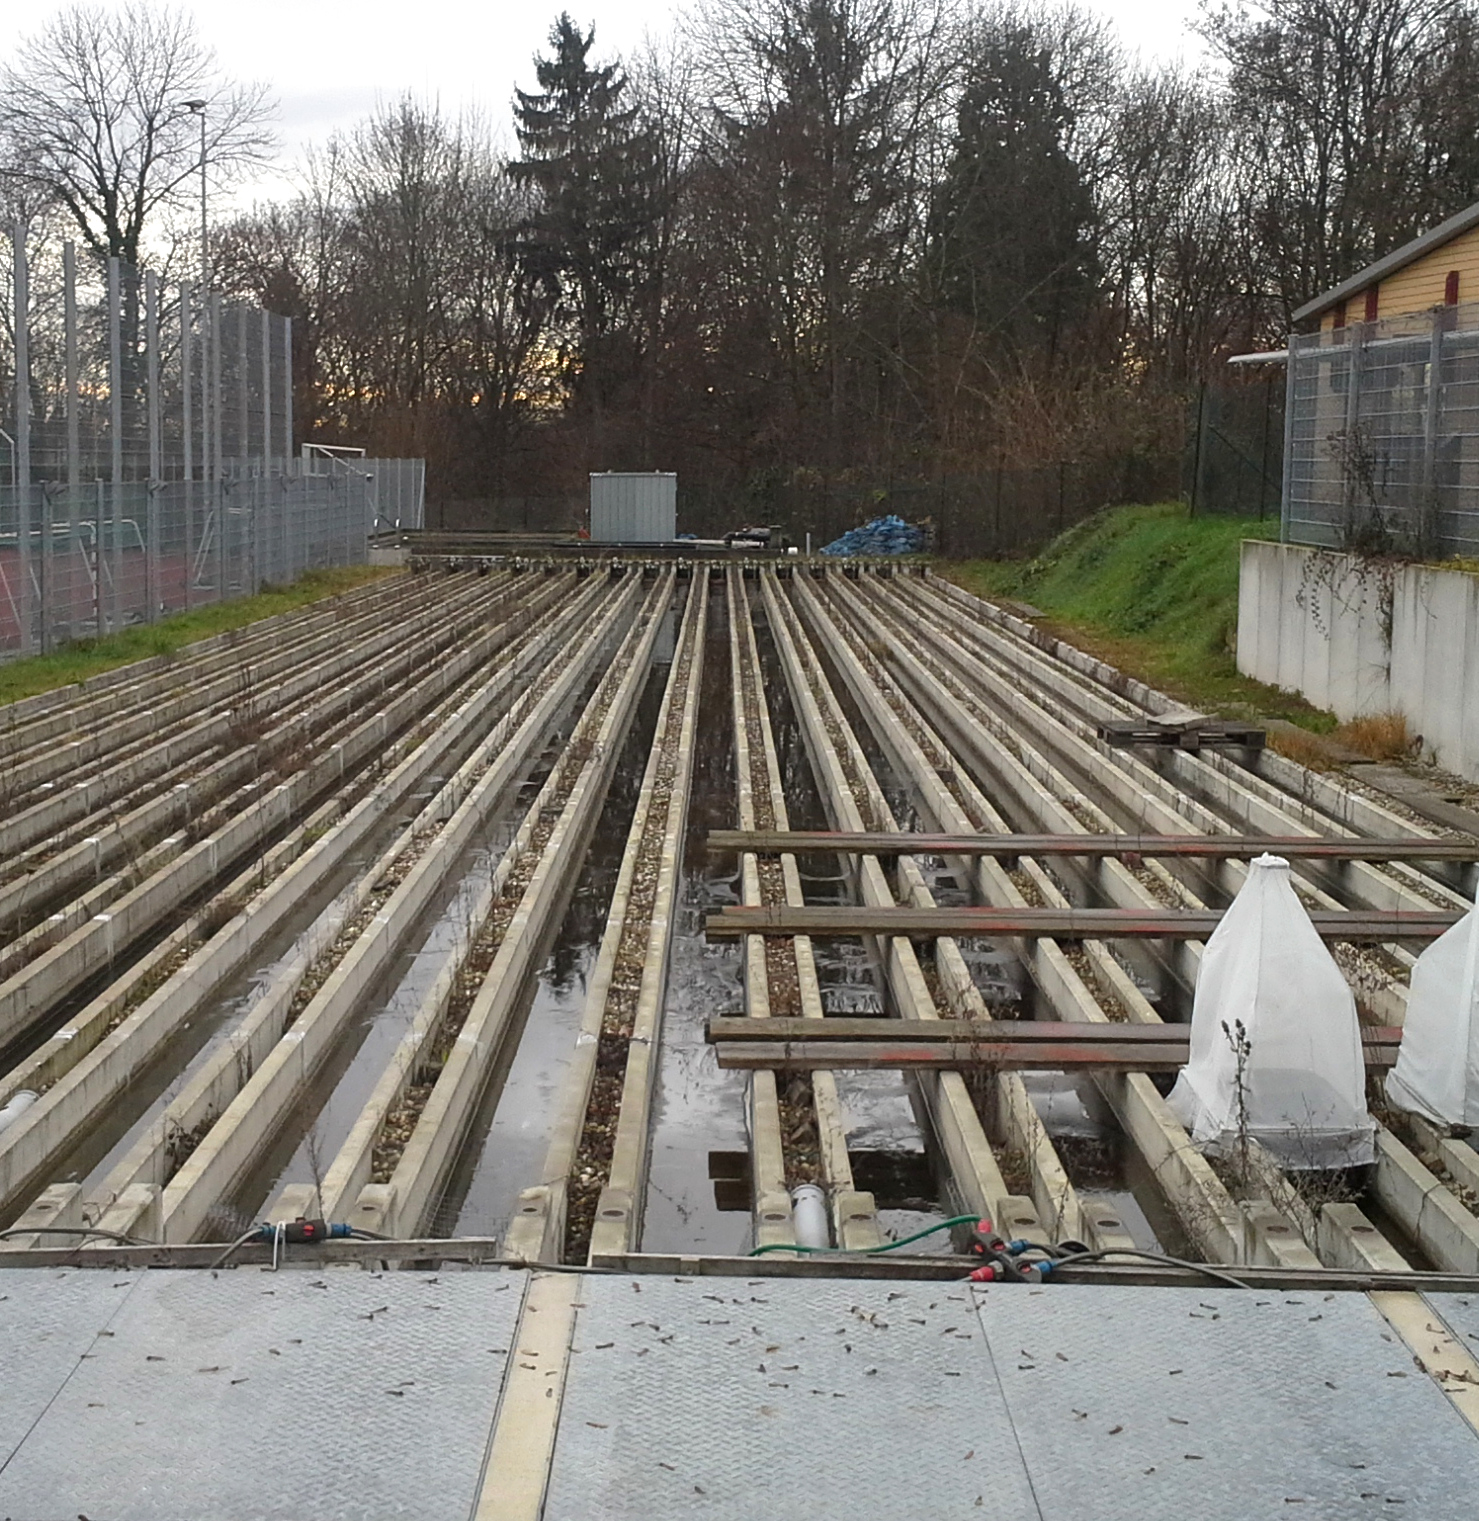
\includegraphics[width=0.9\textwidth]{figs/mesocosm_ld.jpg}
	\end{columns}

	\vfill
	\begin{columns}[T]
	\column<1->{.49\textwidth}
		\begin{itemize}
			\item Daphnia Test
			\item Lower Tier 
			\item \emph{"x out of n survived"}
		\end{itemize}

	\column<2->{.49\textwidth}
		\begin{itemize}
			\item Mesocosm
			\item Higher Tier 
			\item \emph{"number of animals"}
		\end{itemize}
	\end{columns}
\end{frame}
}%



\begin{frame}
\frametitle{Ecotoxicology is not normal}

\begin{columns}[T]
	\column{.49\textwidth}
		\center
		\begin{adjustbox}{max totalsize={0.7\textwidth}{\textheight}}
					\definecolor{myblue}{rgb}{0.137, 0.251, 0.627}
\definecolor{myalert}{rgb}{0.922, 0.482, 0.078}

% overlays etc in tikz
\tikzset{
    invisible/.style={opacity=0},
    visible on/.style={alt={#1{}{invisible}}},
    alt/.code args={<#1>#2#3}{%
      \alt<#1>{\pgfkeysalso{#2}}{\pgfkeysalso{#3}} % \pgfkeysalso doesn't change the path
    },
  }

\begin{tikzpicture}[x=1pt,y=1pt]
%\definecolor{fillColor}{RGB}{255,255,255}
%\path[use as bounding box,fill=fillColor,fill opacity=0.00] (0,0) rectangle (433.62,361.35);
\begin{scope}
\path[clip] ( 18.58, 40.74) rectangle (428.12,355.85);
\path[fill=myblue] ( 37.19, 55.07) rectangle ( 59.09, 55.07);
\path[fill=myblue] ( 80.99, 55.07) rectangle (102.89, 55.14);
\path[fill=myblue] (124.79, 55.07) rectangle (146.70, 56.05);
\path[fill=myblue] (168.60, 55.07) rectangle (190.50, 62.90);
\path[fill=myblue] (212.40, 55.07) rectangle (234.30, 94.23);
\path[fill=myblue] (256.20, 55.07) rectangle (278.10,180.39);
\path[fill=myblue] (300.00, 55.07) rectangle (321.90,305.72);
\path[fill=myblue] (343.80, 55.07) rectangle (365.70,341.53);
\path[fill=myblue] (387.60, 55.07) rectangle (409.50,198.30);
\definecolor{drawColor}{RGB}{0,0,0}
\path[draw=drawColor,line width= 0.6pt,line join=round] ( 18.58, 55.07) -- (428.12, 55.07);
\end{scope}
\begin{scope}
%\path[clip] (  0.00,  0.00) rectangle (433.62,361.35);
\definecolor{drawColor}{gray}{0.30}
\node[text=drawColor,anchor=base,inner sep=0pt, outer sep=0pt, scale=  2.50] at ( 48.14, 18.58) {0};
\node[text=drawColor,anchor=base,inner sep=0pt, outer sep=0pt, scale=  2.50] at ( 91.94, 18.58) {1};
\node[text=drawColor,anchor=base,inner sep=0pt, outer sep=0pt, scale=  2.50] at (135.74, 18.58) {2};
\node[text=drawColor,anchor=base,inner sep=0pt, outer sep=0pt, scale=  2.50] at (179.55, 18.58) {3};
\node[text=drawColor,anchor=base,inner sep=0pt, outer sep=0pt, scale=  2.50] at (223.35, 18.58) {4};
\node[text=drawColor,anchor=base,inner sep=0pt, outer sep=0pt, scale=  2.50] at (267.15, 18.58) {5};
\node[text=drawColor,anchor=base,inner sep=0pt, outer sep=0pt, scale=  2.50] at (310.95, 18.58) {6};
\node[text=drawColor,anchor=base,inner sep=0pt, outer sep=0pt, scale=  2.50] at (354.75, 18.58) {7};
\node[text=drawColor,anchor=base,inner sep=0pt, outer sep=0pt, scale=  2.50] at (398.55, 18.58) {8};
 \node[text=myalert,anchor=base,inner sep=0pt, outer sep=0pt, scale=  4, font=\bf\Huge, rotate=20,
visible on=<2->] at (218, 210) {Normal?};
\end{scope}
\end{tikzpicture}

		\end{adjustbox}
		\begin{itemize}
			\item \emph{"x out of n survived"}
			\onslide<3->{\item<ale@3-> \alert{binomial data}}
		\end{itemize}
	\column{.49\textwidth}
		\center
		\begin{adjustbox}{max totalsize={0.7\textwidth}{\textheight}}
					%\definecolor{myblue}{rgb}{0.137, 0.251, 0.627}
%\definecolor{myalert}{rgb}{0.922, 0.482, 0.078}

% overlays etc in tikz
\tikzset{
    invisible/.style={opacity=0},
    visible on/.style={alt={#1{}{invisible}}},
    alt/.code args={<#1>#2#3}{%
      \alt<#1>{\pgfkeysalso{#2}}{\pgfkeysalso{#3}} % \pgfkeysalso doesn't change the path
    },
  }


\begin{tikzpicture}[x=1pt,y=1pt]
\begin{scope}
% \path[clip] ( 18.58, 40.74) rectangle (428.12,355.85);
\path[fill=myblue] ( 37.19, 55.07) rectangle ( 71.04,198.30);
\path[fill=myblue] (104.88, 55.07) rectangle (138.73,341.53);
\path[fill=myblue] (172.58, 55.07) rectangle (206.42,341.53);
\path[fill=myblue] (240.27, 55.07) rectangle (274.12,246.04);
\path[fill=myblue] (307.96, 55.07) rectangle (341.81,150.55);
\path[fill=myblue] (375.66, 55.07) rectangle (409.50, 93.26);
\definecolor{drawColor}{RGB}{0,0,0}
\path[draw=drawColor,line width= 0.6pt,line join=round] ( 18.58, 55.07) -- (428.12, 55.07);
\end{scope}
\begin{scope}
\definecolor{drawColor}{gray}{0.30}
\node[text=drawColor,anchor=base,inner sep=0pt, outer sep=0pt, scale=  2.50] at ( 54.11, 18.58) {0};
\node[text=drawColor,anchor=base,inner sep=0pt, outer sep=0pt, scale=  2.50] at (121.81, 18.58) {1};
\node[text=drawColor,anchor=base,inner sep=0pt, outer sep=0pt, scale=  2.50] at (189.50, 18.58) {2};
\node[text=drawColor,anchor=base,inner sep=0pt, outer sep=0pt, scale=  2.50] at (257.19, 18.58) {3};
\node[text=drawColor,anchor=base,inner sep=0pt, outer sep=0pt, scale=  2.50] at (324.89, 18.58) {4};
\node[text=drawColor,anchor=base,inner sep=0pt, outer sep=0pt, scale=  2.50] at (392.58, 18.58) {5};
 \node[text=myalert,anchor=base,inner sep=0pt, outer sep=0pt, scale=  4, font=\bf\Huge, rotate=20,
visible on=<2->] at (218, 210) {Normal?};
\end{scope}
\end{tikzpicture}

		\end{adjustbox}
		\begin{itemize}
			\item \emph{"number of animals"}
			\onslide<3->{\item<ale@3-> \alert{count data}}
		\end{itemize}
	\end{columns}

	\onslide<2->{
		\Put(85,50){\begin{adjustbox}{max totalsize={0.9\textwidth}{0.4\textheight}}
			%\definecolor{myblue}{rgb}{0.137, 0.251, 0.627}
%\definecolor{myalert}{rgb}{0.922, 0.482, 0.078}

\begin{tikzpicture}[x=1pt,y=1pt]
\definecolor{fillColor}{RGB}{255,255,255}
%\path[use as bounding box,fill=fillColor,fill opacity=0.00] (0,0) rectangle (433.62,361.35);
\begin{scope}
%\path[clip] ( 18.58, 40.74) rectangle (428.12,355.85);
\path[fill=myblue] ( 37.19, 58.25) --
	( 43.40, 59.34) --
	( 49.60, 60.75) --
	( 55.81, 62.55) --
	( 62.01, 64.82) --
	( 68.22, 67.65) --
	( 74.42, 71.15) --
	( 80.63, 75.41) --
	( 86.83, 80.54) --
	( 93.04, 86.65) --
	( 99.24, 93.84) --
	(105.45,102.18) --
	(111.65,111.76) --
	(117.86,122.60) --
	(124.06,134.71) --
	(130.27,148.07) --
	(136.48,162.58) --
	(142.68,178.12) --
	(148.89,194.50) --
	(155.09,211.50) --
	(161.30,228.81) --
	(167.50,246.13) --
	(173.71,263.08) --
	(179.91,279.28) --
	(186.12,294.34) --
	(192.32,307.87) --
	(198.53,319.50) --
	(204.73,328.92) --
	(210.94,335.85) --
	(217.14,340.10) --
	(223.35,341.53) --
	(229.55,340.10) --
	(235.76,335.85) --
	(241.96,328.92) --
	(248.17,319.50) --
	(254.37,307.87) --
	(260.58,294.34) --
	(266.78,279.28) --
	(272.99,263.08) --
	(279.19,246.13) --
	(285.40,228.81) --
	(291.61,211.50) --
	(297.81,194.50) --
	(304.02,178.12) --
	(310.22,162.58) --
	(316.43,148.07) --
	(322.63,134.71) --
	(328.84,122.60) --
	(335.04,111.76) --
	(341.25,102.18) --
	(347.45, 93.84) --
	(353.66, 86.65) --
	(359.86, 80.54) --
	(366.07, 75.41) --
	(372.27, 71.15) --
	(378.48, 67.65) --
	(384.68, 64.82) --
	(390.89, 62.55) --
	(397.09, 60.75) --
	(403.30, 59.34) --
	(409.50, 58.25) --
	(409.50, 55.07) --
	(403.30, 55.07) --
	(397.09, 55.07) --
	(390.89, 55.07) --
	(384.68, 55.07) --
	(378.48, 55.07) --
	(372.27, 55.07) --
	(366.07, 55.07) --
	(359.86, 55.07) --
	(353.66, 55.07) --
	(347.45, 55.07) --
	(341.25, 55.07) --
	(335.04, 55.07) --
	(328.84, 55.07) --
	(322.63, 55.07) --
	(316.43, 55.07) --
	(310.22, 55.07) --
	(304.02, 55.07) --
	(297.81, 55.07) --
	(291.61, 55.07) --
	(285.40, 55.07) --
	(279.19, 55.07) --
	(272.99, 55.07) --
	(266.78, 55.07) --
	(260.58, 55.07) --
	(254.37, 55.07) --
	(248.17, 55.07) --
	(241.96, 55.07) --
	(235.76, 55.07) --
	(229.55, 55.07) --
	(223.35, 55.07) --
	(217.14, 55.07) --
	(210.94, 55.07) --
	(204.73, 55.07) --
	(198.53, 55.07) --
	(192.32, 55.07) --
	(186.12, 55.07) --
	(179.91, 55.07) --
	(173.71, 55.07) --
	(167.50, 55.07) --
	(161.30, 55.07) --
	(155.09, 55.07) --
	(148.89, 55.07) --
	(142.68, 55.07) --
	(136.48, 55.07) --
	(130.27, 55.07) --
	(124.06, 55.07) --
	(117.86, 55.07) --
	(111.65, 55.07) --
	(105.45, 55.07) --
	( 99.24, 55.07) --
	( 93.04, 55.07) --
	( 86.83, 55.07) --
	( 80.63, 55.07) --
	( 74.42, 55.07) --
	( 68.22, 55.07) --
	( 62.01, 55.07) --
	( 55.81, 55.07) --
	( 49.60, 55.07) --
	( 43.40, 55.07) --
	( 37.19, 55.07) --
	cycle;
\definecolor{drawColor}{RGB}{0,0,0}

\path[draw=drawColor,line width= 0.6pt,line join=round] ( 37.19, 58.25) --
	( 43.40, 59.34) --
	( 49.60, 60.75) --
	( 55.81, 62.55) --
	( 62.01, 64.82) --
	( 68.22, 67.65) --
	( 74.42, 71.15) --
	( 80.63, 75.41) --
	( 86.83, 80.54) --
	( 93.04, 86.65) --
	( 99.24, 93.84) --
	(105.45,102.18) --
	(111.65,111.76) --
	(117.86,122.60) --
	(124.06,134.71) --
	(130.27,148.07) --
	(136.48,162.58) --
	(142.68,178.12) --
	(148.89,194.50) --
	(155.09,211.50) --
	(161.30,228.81) --
	(167.50,246.13) --
	(173.71,263.08) --
	(179.91,279.28) --
	(186.12,294.34) --
	(192.32,307.87) --
	(198.53,319.50) --
	(204.73,328.92) --
	(210.94,335.85) --
	(217.14,340.10) --
	(223.35,341.53) --
	(229.55,340.10) --
	(235.76,335.85) --
	(241.96,328.92) --
	(248.17,319.50) --
	(254.37,307.87) --
	(260.58,294.34) --
	(266.78,279.28) --
	(272.99,263.08) --
	(279.19,246.13) --
	(285.40,228.81) --
	(291.61,211.50) --
	(297.81,194.50) --
	(304.02,178.12) --
	(310.22,162.58) --
	(316.43,148.07) --
	(322.63,134.71) --
	(328.84,122.60) --
	(335.04,111.76) --
	(341.25,102.18) --
	(347.45, 93.84) --
	(353.66, 86.65) --
	(359.86, 80.54) --
	(366.07, 75.41) --
	(372.27, 71.15) --
	(378.48, 67.65) --
	(384.68, 64.82) --
	(390.89, 62.55) --
	(397.09, 60.75) --
	(403.30, 59.34) --
	(409.50, 58.25);

\path[draw=drawColor,line width= 0.6pt,line join=round] ( 18.58, 55.07) -- (428.12, 55.07);
\end{scope}
\begin{scope}
%\path[clip] (  0.00,  0.00) rectangle (433.62,361.35);
\definecolor{drawColor}{gray}{0.30}
\node[text=drawColor,anchor=base,inner sep=0pt, outer sep=0pt, scale=  2.50] at ( 37.19, 18.58) {-1};
\node[text=drawColor,anchor=base,inner sep=0pt, outer sep=0pt, scale=  2.50] at ( 99.24, 18.58) {0};
\node[text=drawColor,anchor=base,inner sep=0pt, outer sep=0pt, scale=  2.50] at (161.30, 18.58) {1};
\node[text=drawColor,anchor=base,inner sep=0pt, outer sep=0pt, scale=  2.50] at (223.35, 18.58) {2};
\node[text=drawColor,anchor=base,inner sep=0pt, outer sep=0pt, scale=  2.50] at (285.40, 18.58) {3};
\node[text=drawColor,anchor=base,inner sep=0pt, outer sep=0pt, scale=  2.50] at (347.45, 18.58) {4};
\node[text=drawColor,anchor=base,inner sep=0pt, outer sep=0pt, scale=  2.50] at (409.50, 18.58) {5};

% \node[text=myalert,anchor=base,inner sep=0pt, outer sep=0pt, scale=  5, font=\bf\Huge, rotate=20] at (218, 300) {Normal?};
\end{scope}
\end{tikzpicture}

		\end{adjustbox}
		}
	}

	\vspace*{1cm}
	\begin{itemize}
		\item<4-> ignore?
		\item<5-> transform?
		\item<6-> non-parametric?
		\only<7>{\item Generalized Linear Model (GLM)}
		\only<8->{\item<ale@2-> \alert{Generalized Linear Model (GLM)}}
	\end{itemize}

\end{frame}



\begin{frame}
\frametitle{A brief history of GLM (uncomprehensive) in ecology}
	% -*- root: ../../talk.tex -*-

%%% GLM History Timeline
% see als http://stackoverflow.com/questions/217834/how-to-create-a-timeline-with-latex


% http://tex.stackexchange.com/questions/55806/mindmap-tikzpicture-in-beamer-reveal-step-by-step/55849#55849
% overlays etc in tikz
\tikzset{
    invisible/.style={opacity=0},
    visible on/.style={alt={#1{}{invisible}}},
    alt/.code args={<#1>#2#3}{%
      \alt<#1>{\pgfkeysalso{#2}}{\pgfkeysalso{#3}} % \pgfkeysalso doesn't change the path
    },
  }


\begin{tikzpicture}[scale=0.57] % timeline 1990-2010->
    % define coordinates (begin, used, end, arrow)
    \foreach \x in {2010,2011,2016, 2017}{
        \pgfmathsetlength\yearposx{(\x-1990)*1cm};
        \coordinate (y\x)   at (\yearposx,0);
        \coordinate (y\x t) at (\yearposx,+3pt);
        \coordinate (y\x b) at (\yearposx,-3pt);
    }
    % draw horizontal line with arrow
    \draw [->] (y2010) -- (y2017);
     \draw[snake] (\yearposx{(2005-1990)*1cm},0) -- (\yearposx{(2010-1990)*1cm},0);


	% Nelder
    \node [ text = myalert,
 visible on=<1>
] at (\yearposx{(2006-1990)*1cm}, 0) [rotate=90,anchor=east] {1972};
    \node [
 visible on=<2->
] at (\yearposx{(2006-1990)*1cm}, 0) [rotate=90,anchor=east] {1972};
    \node [ 
 visible on=<1>
] (nelder) at (\yearposx{(2010-1990)*1cm}, 5)  {
\includegraphics[width=10cm]{/home/edisz/Documents/work/research/projects/2016/1PHD/phd_defense/figs/tikz/glm_hist/nelder.png}};

	% oHara
    \node [ text = myalert,
 visible on=<2>
] at (\yearposx{(2010-1990)*1cm}, 0) [rotate=90,anchor=east] {2010};
    \node [ 
 visible on=<3->
] at (\yearposx{(2010-1990)*1cm}, 0) [rotate=90,anchor=east] {2010};
	\draw  [ 
 visible on=<2->
] (\yearposx{(2010-1990)*1cm}, 3pt) --  (\yearposx{(2010-1990)*1cm}, -3pt);
    \node [ 
 visible on=<2>
] (ohara) at (\yearposx{(2010-1990)*1cm}, 5)  {
\includegraphics[width=10cm]{/home/edisz/Documents/work/research/projects/2016/1PHD/phd_defense/figs/tikz/glm_hist/ohara_2010.png}};

	% warton & Hui
    \node [ text=myalert,
 visible on=<3>
] at (\yearposx{(2011-1990)*1cm}, 0) [rotate=90,anchor=east] {2011};
    \node [ 
 visible on=<4->
] at (\yearposx{(2011-1990)*1cm}, 0) [rotate=90,anchor=east] {2011};
	\draw  [ 
 visible on=<3->
] (\yearposx{(2011-1990)*1cm}, 3pt) --  (\yearposx{(2011-1990)*1cm}, -3pt);
    \node [ 
 visible on=<3>
] (ohara) at (\yearposx{(2010-1990)*1cm}, 5)  {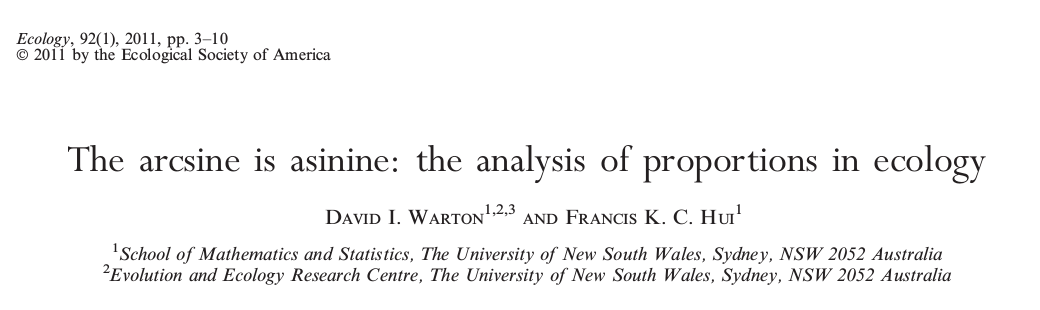
\includegraphics[width=10cm]{/home/edisz/Documents/work/research/projects/2016/1PHD/phd_defense/figs/tikz/glm_hist/warton_2011.png}};

	% warton mvglm
    \node [ text=myalert,
 visible on=<4>
] at (\yearposx{(2012-1990)*1cm}, 0) [rotate=90,anchor=east] {2012};
    \node [ 
 visible on=<5->
] at (\yearposx{(2012-1990)*1cm}, 0) [rotate=90,anchor=east] {2012};
	\draw  [ 
 visible on=<4->
] (\yearposx{(2012-1990)*1cm}, 3pt) --  (\yearposx{(2012-1990)*1cm}, -3pt);
    \node [ 
 visible on=<4>
] (ohara) at (\yearposx{(2010-1990)*1cm}, 5)  {
\includegraphics[width=10cm]{/home/edisz/Documents/work/research/projects/2016/1PHD/phd_defense/figs/tikz/glm_hist/warton_2012.png}};

	% Szoecs, mesocosm
    \node [ text=myalert,
 visible on=<5->
] at (\yearposx{(2015-1990)*1cm}, 0) [rotate=90,anchor=east] {2015};
	\draw  [ 
 visible on=<5->
] (\yearposx{(2015-1990)*1cm}, 3pt) --  (\yearposx{(2015-1990)*1cm}, -3pt);
    \node [ 
 visible on=<5>
] (ohara) at (\yearposx{(2010-1990)*1cm}, 5)  {
\includegraphics[width=10cm]{/home/edisz/Documents/work/research/projects/2016/1PHD/phd_defense/figs/tikz/glm_hist/Szoecs_2015.png}};

	% Szoecs, normal
    \node [ 
 visible on=<6>
] (ohara) at (\yearposx{(2010-1990)*1cm}, 5)  {
\includegraphics[width=10cm]{/home/edisz/Documents/work/research/projects/2016/1PHD/phd_defense/figs/tikz/glm_hist/Szoecs_2015_notnormal.png}};


\end{tikzpicture}

\end{frame}



\begin{frame}
\frametitle{A simulation study}

\end{frame}



\begin{frame}
\frametitle{Statistical Power is unacceptably low}

\end{frame}


\begin{frame}
\frametitle{GLM can do better}

\end{frame}



\begin{frame}
\frametitle{What we learned}

\end{frame}


\begin{frame}
\frametitle{Where are we today?}
	% -*- root: ../../talk.tex -*-

%%% GLM History Timeline
% see als http://stackoverflow.com/questions/217834/how-to-create-a-timeline-with-latex


% http://tex.stackexchange.com/questions/55806/mindmap-tikzpicture-in-beamer-reveal-step-by-step/55849#55849
% overlays etc in tikz
\tikzset{
    invisible/.style={opacity=0},
    visible on/.style={alt={#1{}{invisible}}},
    alt/.code args={<#1>#2#3}{%
      \alt<#1>{\pgfkeysalso{#2}}{\pgfkeysalso{#3}} % \pgfkeysalso doesn't change the path
    },
  }


\begin{tikzpicture}[scale=0.57] % timeline 1990-2010->
    % define coordinates (begin, used, end, arrow)
    \foreach \x in {2010,2011,2016, 2017}{
        \pgfmathsetlength\yearposx{(\x-1990)*1cm};
        \coordinate (y\x)   at (\yearposx,0);
        \coordinate (y\x t) at (\yearposx,+3pt);
        \coordinate (y\x b) at (\yearposx,-3pt);
    }
    % draw horizontal line with arrow
    \draw [->] (y2010) -- (y2017);
     \draw[snake] (\yearposx{(2005-1990)*1cm},0) -- (\yearposx{(2010-1990)*1cm},0);

	% Nelder
    \node [ 
 visible on=<1->
] at (\yearposx{(2006-1990)*1cm}, 0) [rotate=90,anchor=east] {1972};

	% oHara
    \node [ 
 visible on=<1->
] at (\yearposx{(2010-1990)*1cm}, 0) [rotate=90,anchor=east] {2010};
	\draw  [ 
 visible on=<1->
] (\yearposx{(2010-1990)*1cm}, 3pt) --  (\yearposx{(2010-1990)*1cm}, -3pt);


	% warton & Hui
    \node [ 
 visible on=<1->
] at (\yearposx{(2011-1990)*1cm}, 0) [rotate=90,anchor=east] {2011};
	\draw  [ 
 visible on=<1->
] (\yearposx{(2011-1990)*1cm}, 3pt) --  (\yearposx{(2011-1990)*1cm}, -3pt);

	% warton mvglm
    \node [ 
 visible on=<1->
] at (\yearposx{(2012-1990)*1cm}, 0) [rotate=90,anchor=east] {2012};
	\draw  [ 
 visible on=<1->
] (\yearposx{(2012-1990)*1cm}, 3pt) --  (\yearposx{(2012-1990)*1cm}, -3pt);

	% Szoecs, mesocosm
    \node [ text = myalert,
 visible on=<1>
] at (\yearposx{(2015-1990)*1cm}, 0) [rotate=90,anchor=east] {2015};
    \node [
 visible on=<2->
] at (\yearposx{(2015-1990)*1cm}, 0) [rotate=90,anchor=east] {2015};
	\draw  [ 
 visible on=<1->
] (\yearposx{(2015-1990)*1cm}, 3pt) --  (\yearposx{(2015-1990)*1cm}, -3pt);

	% Ives
    \node [ 
 visible on=<1>
] (ohara) at (\yearposx{(2010-1990)*1cm}, 5)  {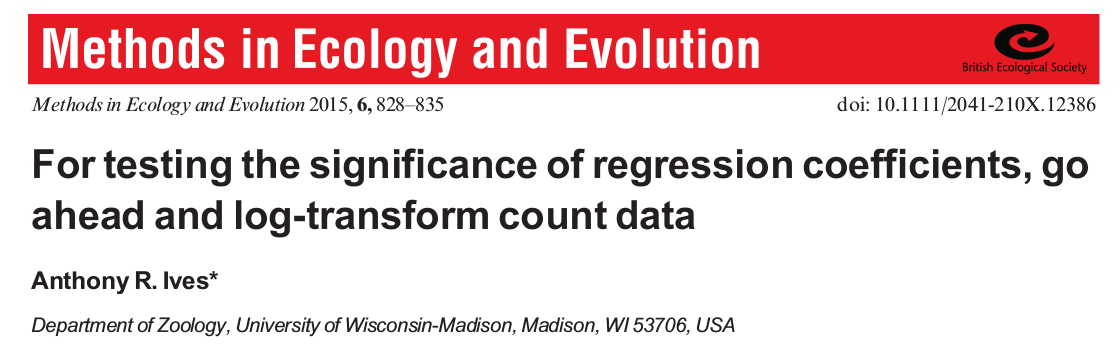
\includegraphics[width=10cm]{/home/edisz/Documents/work/research/projects/2016/1PHD/phd_defense/figs/tikz/glm_hist/ives_2015.png}};

	% warton
    \node [ text = myalert,
 visible on=<2->
] at (\yearposx{(2016-1990)*1cm}, 0) [rotate=90,anchor=east] {2016};
	\draw  [ 
 visible on=<2->
] (\yearposx{(2016-1990)*1cm}, 3pt) --  (\yearposx{(2016-1990)*1cm}, -3pt);
    \node [ 
 visible on=<2->
] (ohara) at (\yearposx{(2010-1990)*1cm}, 5)  {
\includegraphics[width=10cm]{/home/edisz/Documents/work/research/projects/2016/1PHD/phd_defense/figs/tikz/glm_hist/warton_2016.png}};


\end{tikzpicture}

\end{frame}


{%
\setbeamertemplate{frame footer}{Warton, D.I., Lyons, M., Stoklosa, J., Ives, A.R., 2016. Three points to consider when choosing a LM or GLM test for count data. Methods in Ecology and Evolution 7, 882–890.
}
\begin{frame}
\frametitle{Where are we today?}
	% \metroset{block=fill}
	\begin{exampleblock}{Three points to consider ...}
		\begin{enumerate}
			\item Choose your model based on data properties
			\item Fix Type I errors by resampling
			\item Models that better fit the data have better power properties
		\end{enumerate}
	\end{exampleblock}
\end{frame}
}

%%% ---------------------------------------------------------------------------
\section{Exploring Monitoring Data for ERA}

\begin{frame}
\frametitle{Environmental Monitoring}

\end{frame}

\begin{frame}
\frametitle{Overview on data compiled}

\end{frame}

\begin{frame}
\frametitle{Thresholds}

\end{frame}

\begin{frame}
\frametitle{Statistics with chemical measurements}

\end{frame}


\begin{frame}
\frametitle{Dynamics}

\end{frame}


\begin{frame}
\frametitle{Risks}
Check: What did go wrong with Neonics during ERA?
Exposure wromg? Effect wrong (e.g. did not consider sensitive species)?
=> Quite sure that Effect assessment missed it...
=> show SSD, highlighting standard test species (from EPA)
* old guidance document did not enforce insect.
* new one (from 2013) enforces additional insect data

RAC is landscape dependend (=> exposure?)

Example for power (experimental setup)

\end{frame}


\begin{frame}
\frametitle{What we learned}

\end{frame}

%%% ---------------------------------------------------------------------------
\section{Solutions for Linking Data in ERA}

\begin{frame}
\frametitle{Biologists \& Chemists face the same problems}
	\small
	\centering
	\textbf{\alert{\underline{Names}}}
	\begin{columns}[t]
	\column{.45\textwidth}
	\emph{Osmia rufa, Osmia bicornis, Osmia ruffa, Osmia unilandauis, Osmia spec.} 
	\column{.45\textwidth}
	Chlorpyrifos, Chlorpyriphos, Chlorphyrifos, Chlorpyrifos-ethyl, Chlorpypifot
	\end{columns}
	\pause

	\centering
	\textbf{\alert{\underline{Hierarchies}}}
	\begin{columns}[t]
	\column{.45\textwidth}
	Hymenoptera/ Apoidea/ Megachilidae/ Osmia/ rufa 
	\column{.45\textwidth}
	organophospate, ester, insecticide
	\end{columns}
	\pause

	\centering
	\textbf{\alert{\underline{Traits / Properties}}}
	\begin{columns}[t]
	\column{.45\textwidth}
	Wing length, Mass, Season 
	\column{.45\textwidth}
	Mass, $K_{OW}$, $LC_{50}$
	\end{columns}
	\pause

	\centering
	\textbf{\alert{\underline{Identifiers}}}
	\begin{columns}[t]
	\column{.45\textwidth}
	NCBI, ITIS, EOL, ... 
	\column{.45\textwidth}
	2921-88-2, Clc1c(OP(=S)[...], InChI=1S/C9H11C[...], SBPBAQFW[...], CSID,...
	\end{columns}
	\vspace{0.8em}
	\pause

	\rule{\textwidth}{1pt}
	\textbf{\alert{\underline{Amount of data}}}

	\begin{columns}[t]
	\column{.45\textwidth}
	\centering
	2993 taxa
	\column{.45\textwidth}
	\centering
	489 pesticides \\ (+ 590 other organics)
	\end{columns}
\end{frame}


{%
\setbeamertemplate{frame footer}{Münch et al. (2016). DoOR 2.0 - Comprehensive Mapping of Drosophila melanogaster Odorant Responses. Scientific Reports 6, 21841
}
\begin{frame}{}
\frametitle{Instead of wasting time...}
... use \alert{webchem}! \\
	\hspace*{2cm}
	\begin{adjustbox}{max totalsize={\textwidth}{0.8\textheight}}
				% -*- root: ../../talk.tex -*-

\definecolor{blue}{RGB}{32, 126, 153}
\definecolor{green}{RGB}{33, 182, 78}
\definecolor{red}{RGB}{246, 72, 45}
\definecolor{orange}{RGB}{246, 146, 45}
\definecolor{yellow}{RGB}{180, 180, 18}

\begin{tikzpicture}[node distance = 0.2cm, auto]

%styles
\tikzstyle{circ} = [circle, draw, text = black,   line width=1pt, 
    text width=4cm, text centered, scale=1, font=\bf\huge]
\tikzstyle{rect} = [rectangle, draw, text = black, line width=1pt,
    text width=5cm, text centered, rounded corners, minimum height=1.5cm, minimum width=1cm, font=\bf\huge]

\tikzstyle{line} = [draw, -{Latex[length=5mm,width=3mm]}, line width=1mm, opacity = 0.8]

    % input nodes
    \node [circ, fill=green] (cas_i) {CAS};
    \node  (name_i) [circ, below=of cas_i, fill = blue] {Name};
    \node  (inchikey_i) [circ, below=of name_i, fill = red] {InChiKey};
    \node  (other_i) [circ, below=of inchikey_i, fill =orange] {Other};
   
   % source nodes
   \node (cir) [rect, right=of cas_i, shift={(13,7)}, fill = yellow]{CIR};
   \node (chemspider) [rect, below=1cm of cir, fill = yellow]{ChemSpider};
   \node (cts) [rect, below=1cm of chemspider, fill = yellow]{CTS};
   \node (etox) [rect, below=1cm of cts, fill = yellow]{ETOX};
   \node (chemid) [rect, below=1cm of etox, fill = yellow]{ChemID};
  \node (opsin) [rect, below=1cm of chemid, fill = yellow]{OPSIN};
  \node (alan) [rect, below=1cm of opsin, fill = yellow]{Pesticide Compendium};
  \node (wiki) [rect, below=1cm of alan, fill = yellow]{wikidata};
  \node (pubchem) [rect, below=1cm of wiki, fill = yellow]{PubChem};
  \node (pan) [rect, below=1cm of pubchem, fill = yellow]{PAN};
  \node (src) [rect, below=1cm of pan, fill = yellow]{SRC};

	% output nodes
    \node (cas_o) [circ, right=of cir, shift={(15,-5)}, , fill =green] {CAS};
    \node  (name_o) [circ, below=of cas_o, , fill =blue] {Name};
    \node  (inchikey_o) [circ, below=of name_o, fill =red] {InChiKey \\ InChi};
    \node  (smiles_o) [circ, below=of inchikey_o, fill =red] {SMILES};
    \node  (legis_o) [circ, below=of smiles_o, fill =orange] {Legislation};
    \node  (syno_o) [circ, below=of legis_o, fill =orange] {Synonyms};
    \node  (other_o) [circ, below=of syno_o, fill =orange] {Other};
    \node (prop_o) [circ, above=of cas_o, fill =orange] {Properties};
    \node (tox_o) [circ, above=of prop_o, fill =orange] {Toxicology};

    %paths
   % from cas_i
    \path [line, green] (cas_i.east) -- (cir.west);
    \path [line, green] (cas_i.east) -- (chemspider.west);
    \path [line, green] (cas_i.east) -- (cts.west);
    \path [line, green] (cas_i.east) -- (etox.west);
    \path [line, green] (cas_i.east) -- (chemid.west);
    \path [line, green] (cas_i.east) -- (alan.west);
    \path [line, green] (cas_i.east) -- (wiki.west);
    \path [line, green] (cas_i.east) -- (pubchem.west);
    \path [line, green] (cas_i.east) -- (pan.west);
    \path [line, green] (cas_i.east) -- (src.west);

	% from name_i
    \path [line, blue] (name_i.east) -- (cir.west);
    \path [line, blue] (name_i.east) -- (chemspider.west);
    \path [line, blue] (name_i.east) -- (cts.west);
    \path [line, blue] (name_i.east) -- (etox.west);
    \path [line, blue] (name_i.east) -- (chemid.west);
    \path [line, blue] (name_i.east) -- (opsin.west);
    \path [line, blue] (name_i.east) -- (alan.west);
    \path [line, blue] (name_i.east) -- (wiki.west);
    \path [line, blue] (name_i.east) -- (pubchem.west);
    \path [line, blue] (name_i.east) -- (pan.west);

    %from inchikey_i
    \path [line, red] (inchikey_i.east) -- (cir.west);
    \path [line, red] (inchikey_i.east) -- (chemspider.west);
    \path [line, red] (inchikey_i.east) -- (cts.west);
    \path [line, red] (inchikey_i.east) -- (chemid.west);
    \path [line, red] (inchikey_i.east) -- (wiki.west);
    \path [line, red] (inchikey_i.east) -- (pubchem.west);
   
    %from other_i
    \path [line, orange] (other_i.east) -- (cir.west);
    \path [line, orange] (other_i.east) -- (chemspider.west);
    \path [line, orange] (other_i.east) -- (cts.west);
    \path [line, orange] (other_i.east) -- (etox.west);
    \path [line, orange] (other_i.east) -- (wiki.west);
    \path [line, orange] (other_i.east) -- (pubchem.west);

   %from cir
  \path [line, orange] (cir.east) -- (prop_o.west);
  \path [line, green] (cir.east) -- (cas_o.west);
  \path [line, blue] (cir.east) -- (name_o.west);
  \path [line, red] (cir.east) -- (inchikey_o.west);
  \path [line, red] (cir.east) -- (smiles_o.west);
  \path [line, orange] (cir.east) -- (other_o.west);

  %from chemspider
  \path [line, orange] (chemspider.east) -- (prop_o.west);
  \path [line, blue] (chemspider.east) -- (name_o.west);
  \path [line, red] (chemspider.east) -- (inchikey_o.west);
  \path [line, red] (chemspider.east) -- (smiles_o.west);

  % from cts
  \path [line, blue] (cts.east) -- (name_o.west);
  \path [line, green] (cts.east) -- (cas_o.west);
  \path [line, red] (cts.east) -- (inchikey_o.west);
  \path [line, red] (cts.east) -- (smiles_o.west);
  \path [line, orange] (cts.east) -- (syno_o.west);
  \path [line, orange] (cts.east) -- (other_o.west);

	% from etox
   \path [line, orange] (etox.east) -- (tox_o.west);
   \path [line, green] (etox.east) -- (cas_o.west);
   \path [line, blue] (etox.east) -- (name_o.west);
   \path [line, orange] (etox.east) -- (legis_o.west);
   \path [line, orange] (etox.east) -- (syno_o.west);
   \path [line, orange] (etox.east) -- (other_o.west);

  %from chemid
   \path [line, orange] (chemid.east) -- (tox_o.west);
   \path [line, orange] (chemid.east) -- (prop_o.west);
   \path [line, green] (chemid.east) -- (cas_o.west);
   \path [line, blue] (chemid.east) -- (name_o.west);
   \path [line, red] (chemid.east) -- (inchikey_o.west);
   \path [line, red] (chemid.east) -- (smiles_o.west);
   \path [line, orange] (chemid.east) -- (syno_o.west);

	%from opsin
    \path [line, green] (opsin.east) -- (cas_o.west);
   \path [line, red] (opsin.east) -- (inchikey_o.west);
   \path [line, red] (opsin.east) -- (smiles_o.west);

   %from alan wood
   \path [line, green] (alan.east) -- (cas_o.west);
   \path [line, blue] (alan.east) -- (name_o.west);
   \path [line, red] (alan.east) -- (inchikey_o.west);
   \path [line, orange] (alan.east) -- (other_o.west);

  %from wiki
   \path [line, green] (wiki.east) -- (cas_o.west);
   \path [line, red] (wiki.east) -- (inchikey_o.west);
   \path [line, red] (wiki.east) -- (smiles_o.west);
   \path [line, orange] (wiki.east) -- (other_o.west);

  % from pubchem
     \path [line, orange] (pubchem.east) -- (prop_o.west);
     \path [line, blue] (pubchem.east) -- (name_o.west);
     \path [line, red] (pubchem.east) -- (inchikey_o.west);
     \path [line, red] (pubchem.east) -- (smiles_o.west);
     \path [line, orange] (pubchem.east) -- (syno_o.west);

    % from pan
    \path [line, orange] (pan.east) -- (tox_o.west);
    \path [line, orange] (pan.east) -- (prop_o.west);
     \path [line, blue] (pan.east) -- (name_o.west);
   \path [line, green] (pan.east) -- (cas_o.west);
   \path [line, orange] (pan.east) -- (legis_o.west);
   \path [line, orange] (pan.east) -- (other_o.west);

  %from src
       \path [line, orange] (src.east) -- (tox_o.west);
     \path [line, blue] (src.east) -- (name_o.west);
   \path [line, green] (src.east) -- (cas_o.west);

\end{tikzpicture}

	\end{adjustbox}

\pause
\vspace*{-1cm}\emph{''\alert{webchem} ...likely saved hundreds of working hours''}
\end{frame}
}


{%
\setbeamertemplate{frame footer}{Dr. Susan E. Johnston, University of Edinburgh. On twitter.
}
\begin{frame}
\frametitle{Instead of wasting time...}
... use \alert{taxize!} \\
	\hspace*{-2cm}
	\begin{center}
	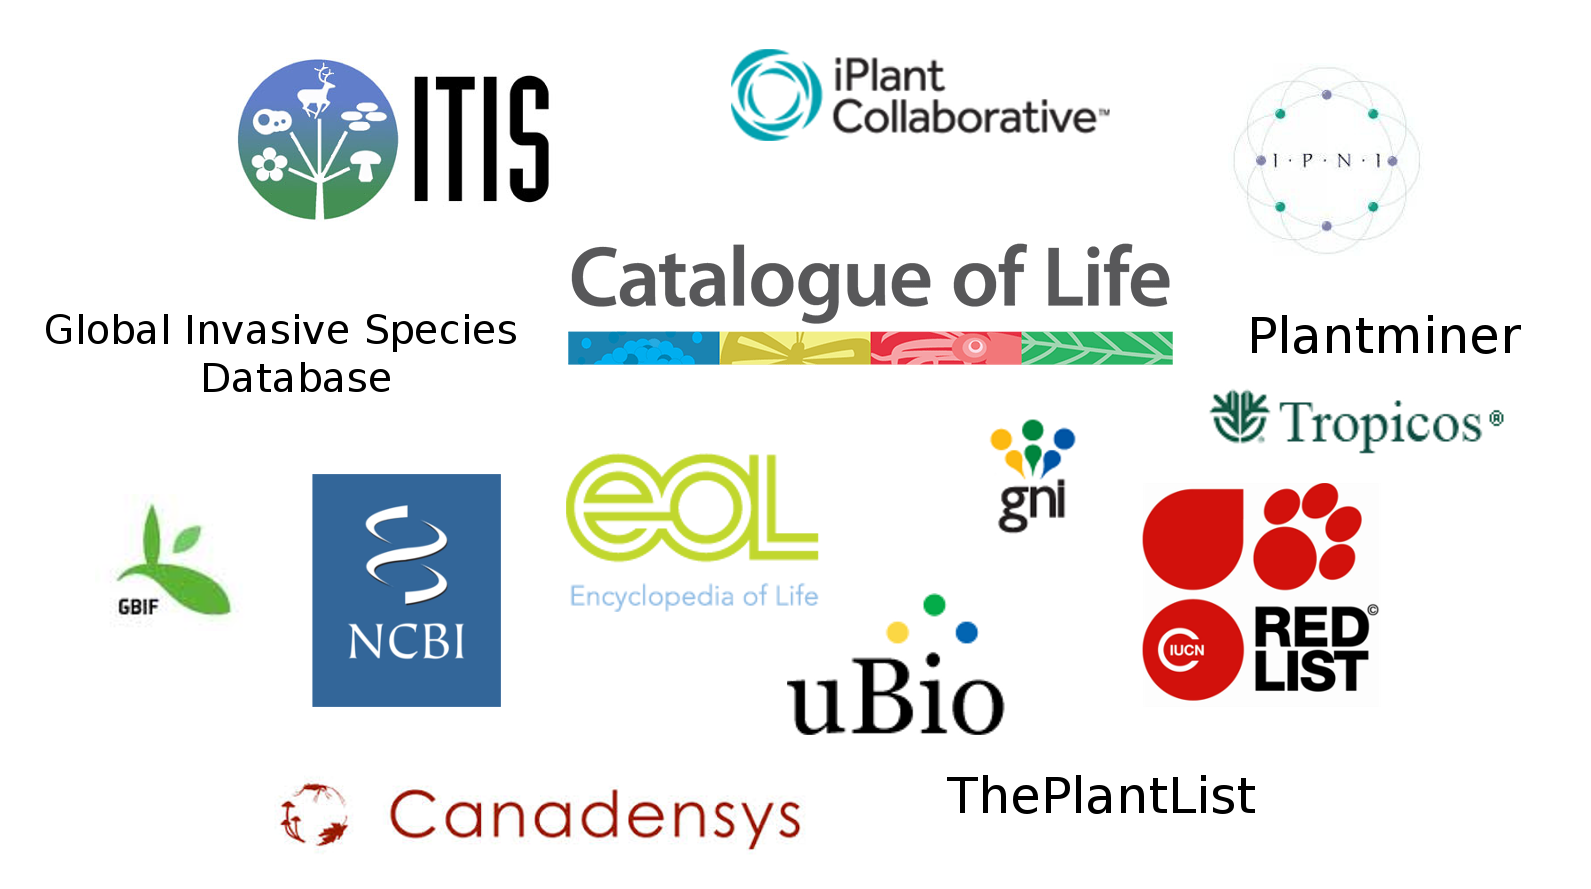
\includegraphics[height=0.6\textheight]{figs/sources_taxize.png}
	\end{center}

\pause
\emph{''Days of searching done during my morning coffee. Amazing. \alert{taxize}.''}
\end{frame}
}



%%% ---------------------------------------------------------------------------
\section*{Recap}

\begin{frame}
\frametitle{What we learned}
	\metroset{block=fill}
	\begin{exampleblock}{\checkmark Improving Statistics in ERA}
		\begin{itemize}
			\item Change your model, not your data
			\item Ultimately ban NOEC
			\item Take LOQ into account
		\end{itemize}
	\end{exampleblock}

\pause
	\begin{exampleblock}{\checkmark Exploring Monitoring Data for ERA}
		\begin{itemize}
			\item Pesticide Dynamics
			\item Agricultural small streams at risk
			\item Neonicotinoids
			\item Feedback for ERA
		\end{itemize}
	\end{exampleblock}

\pause
	\begin{exampleblock}{\checkmark Solutions for Linking Data in ERA}
		\begin{itemize}
			\item Handling big eco(toxico-)logical data not easy
			\item Now easier
		\end{itemize}
	\end{exampleblock}


\end{frame}


%%% ---------------------------------------------------------------------------
%%% Final slide
\begin{frame}[standout]
	\frametitle{}

	\vspace{1em}
	\Huge{Statistical Ecotoxicology} \\[0.3em]
	\large{Improving the Utilisation of Data for \\ Environmental Risk Assessment} \\[1em]

	\normalsize
	Eduard Szöcs \\[3em]

	\faLaptop~~~\textbf{\href{http://edild.github.io/}{http://edild.github.io/ }}\\[.5em]
	\faTwitter~~~\textbf{\href{http://twitter.com/EduardSzoecs}{@EduardSzoecs}} 	\\[0.5em]
	\faFilePowerpointO~~~\textbf{\href{https://github.com/edild/phd_defense}{https://github.com/edild/phd\_defense}}\\[0.5em]
	\faBook~~~\textbf{\href{https://github.com/edild/phd_thesis}{https://github.com/edild/phd\_thesis}}\\[3em]

	\begin{center}\ccbysa\end{center} 

\end{frame}


\appendix

\begin{frame}
\frametitle{Statistics?}

\end{frame}


\begin{frame}
\frametitle{ZAGA what...?}

\end{frame}


\begin{frame}
\frametitle{Comparison with Stehle / Knauer?}

\end{frame}


\begin{frame}
\frametitle{RACs by Type}
	\begin{adjustbox}{max totalsize={\textwidth}{0.95\textheight}}
				% Created by tikzDevice version 0.10.1 on 2016-12-09 10:11:42
% !TEX encoding = UTF-8 Unicode
\begin{tikzpicture}[x=1pt,y=1pt]
\definecolor{fillColor}{RGB}{255,255,255}
\path[use as bounding box,fill=fillColor,fill opacity=0.00] (0,0) rectangle (505.89,361.35);
\begin{scope}
\path[clip] (  0.00,  0.00) rectangle (505.89,361.35);
\definecolor{drawColor}{RGB}{255,255,255}
\definecolor{fillColor}{RGB}{255,255,255}

\path[draw=drawColor,line width= 0.6pt,line join=round,line cap=round,fill=fillColor] (  0.00,  0.00) rectangle (505.89,361.35);
\end{scope}
\begin{scope}
\path[clip] ( 87.99, 41.00) rectangle (498.89,332.44);
\definecolor{fillColor}{RGB}{255,255,255}

\path[fill=fillColor] ( 87.99, 41.00) rectangle (498.89,332.44);
\definecolor{drawColor}{gray}{0.90}

\path[draw=drawColor,line width= 0.6pt,line join=round] ( 87.99, 68.70) --
	(498.89, 68.70);

\path[draw=drawColor,line width= 0.6pt,line join=round] ( 87.99,110.22) --
	(498.89,110.22);

\path[draw=drawColor,line width= 0.6pt,line join=round] ( 87.99,151.73) --
	(498.89,151.73);

\path[draw=drawColor,line width= 0.6pt,line join=round] ( 87.99,193.25) --
	(498.89,193.25);

\path[draw=drawColor,line width= 0.6pt,line join=round] ( 87.99,234.77) --
	(498.89,234.77);

\path[draw=drawColor,line width= 0.6pt,line join=round] ( 87.99,276.28) --
	(498.89,276.28);

\path[draw=drawColor,line width= 0.6pt,line join=round] ( 87.99,317.80) --
	(498.89,317.80);

\path[draw=drawColor,line width= 0.6pt,line join=round] (146.69, 41.00) --
	(146.69,332.44);

\path[draw=drawColor,line width= 0.6pt,line join=round] (244.52, 41.00) --
	(244.52,332.44);

\path[draw=drawColor,line width= 0.6pt,line join=round] (342.36, 41.00) --
	(342.36,332.44);

\path[draw=drawColor,line width= 0.6pt,line join=round] (440.19, 41.00) --
	(440.19,332.44);
\definecolor{drawColor}{gray}{0.20}
\definecolor{fillColor}{gray}{0.20}

\path[draw=drawColor,line width= 0.4pt,line join=round,line cap=round,fill=fillColor] (146.69,287.76) circle (  1.96);

\path[draw=drawColor,line width= 0.6pt,line join=round] (146.69,222.59) -- (146.69,262.28);

\path[draw=drawColor,line width= 0.6pt,line join=round] (146.69,179.62) -- (146.69,130.96);
\definecolor{fillColor}{gray}{0.75}

\path[draw=drawColor,line width= 0.6pt,line join=round,line cap=round,fill=fillColor] (110.00,222.59) --
	(110.00,179.62) --
	(183.38,179.62) --
	(183.38,222.59) --
	(110.00,222.59) --
	cycle;

\path[draw=drawColor,line width= 1.1pt,line join=round] (110.00,194.11) -- (183.38,194.11);
\definecolor{fillColor}{gray}{0.20}

\path[draw=drawColor,line width= 0.4pt,line join=round,line cap=round,fill=fillColor] (244.52,319.19) circle (  1.96);

\path[draw=drawColor,line width= 0.6pt,line join=round] (244.52,238.05) -- (244.52,306.52);

\path[draw=drawColor,line width= 0.6pt,line join=round] (244.52,187.24) -- (244.52,126.74);
\definecolor{fillColor}{gray}{0.75}

\path[draw=drawColor,line width= 0.6pt,line join=round,line cap=round,fill=fillColor] (207.84,238.05) --
	(207.84,187.24) --
	(281.21,187.24) --
	(281.21,238.05) --
	(207.84,238.05) --
	cycle;

\path[draw=drawColor,line width= 1.1pt,line join=round] (207.84,205.75) -- (281.21,205.75);
\definecolor{fillColor}{gray}{0.20}

\path[draw=drawColor,line width= 0.4pt,line join=round,line cap=round,fill=fillColor] (342.36,296.68) circle (  1.96);

\path[draw=drawColor,line width= 0.6pt,line join=round] (342.36,179.24) -- (342.36,234.77);

\path[draw=drawColor,line width= 0.6pt,line join=round] (342.36,101.26) -- (342.36, 54.30);
\definecolor{fillColor}{gray}{0.75}

\path[draw=drawColor,line width= 0.6pt,line join=round,line cap=round,fill=fillColor] (305.67,179.24) --
	(305.67,101.26) --
	(379.04,101.26) --
	(379.04,179.24) --
	(305.67,179.24) --
	cycle;

\path[draw=drawColor,line width= 1.1pt,line join=round] (305.67,134.13) -- (379.04,134.13);

\path[draw=drawColor,line width= 0.6pt,line join=round] (440.19,246.37) -- (440.19,286.88);

\path[draw=drawColor,line width= 0.6pt,line join=round] (440.19,210.62) -- (440.19,194.97);

\path[draw=drawColor,line width= 0.6pt,line join=round,line cap=round,fill=fillColor] (403.50,246.37) --
	(403.50,210.62) --
	(476.88,210.62) --
	(476.88,246.37) --
	(403.50,246.37) --
	cycle;

\path[draw=drawColor,line width= 1.1pt,line join=round] (403.50,224.35) -- (476.88,224.35);
\definecolor{drawColor}{RGB}{0,0,0}
\definecolor{fillColor}{RGB}{0,0,0}

\path[draw=drawColor,line width= 0.4pt,line join=round,line cap=round,fill=fillColor] (454.28,194.99) circle (  1.96);

\path[draw=drawColor,line width= 0.4pt,line join=round,line cap=round,fill=fillColor] (450.89,232.93) circle (  1.96);

\path[draw=drawColor,line width= 0.4pt,line join=round,line cap=round,fill=fillColor] (336.02,167.55) circle (  1.96);

\path[draw=drawColor,line width= 0.4pt,line join=round,line cap=round,fill=fillColor] (234.91,194.27) circle (  1.96);

\path[draw=drawColor,line width= 0.4pt,line join=round,line cap=round,fill=fillColor] (141.99,182.49) circle (  1.96);

\path[draw=drawColor,line width= 0.4pt,line join=round,line cap=round,fill=fillColor] (132.00,247.20) circle (  1.96);

\path[draw=drawColor,line width= 0.4pt,line join=round,line cap=round,fill=fillColor] (257.31,306.53) circle (  1.96);

\path[draw=drawColor,line width= 0.4pt,line join=round,line cap=round,fill=fillColor] (338.11, 56.14) circle (  1.96);

\path[draw=drawColor,line width= 0.4pt,line join=round,line cap=round,fill=fillColor] (157.51,179.23) circle (  1.96);

\path[draw=drawColor,line width= 0.4pt,line join=round,line cap=round,fill=fillColor] (136.20,238.79) circle (  1.96);

\path[draw=drawColor,line width= 0.4pt,line join=round,line cap=round,fill=fillColor] (250.95,214.79) circle (  1.96);

\path[draw=drawColor,line width= 0.4pt,line join=round,line cap=round,fill=fillColor] (159.92,222.31) circle (  1.96);

\path[draw=drawColor,line width= 0.4pt,line join=round,line cap=round,fill=fillColor] (130.01,159.02) circle (  1.96);

\path[draw=drawColor,line width= 0.4pt,line join=round,line cap=round,fill=fillColor] (259.30,172.10) circle (  1.96);

\path[draw=drawColor,line width= 0.4pt,line join=round,line cap=round,fill=fillColor] (348.87,174.51) circle (  1.96);

\path[draw=drawColor,line width= 0.4pt,line join=round,line cap=round,fill=fillColor] (242.04,265.81) circle (  1.96);

\path[draw=drawColor,line width= 0.4pt,line join=round,line cap=round,fill=fillColor] (437.47,215.90) circle (  1.96);

\path[draw=drawColor,line width= 0.4pt,line join=round,line cap=round,fill=fillColor] (341.51, 54.25) circle (  1.96);

\path[draw=drawColor,line width= 0.4pt,line join=round,line cap=round,fill=fillColor] (261.29,208.26) circle (  1.96);

\path[draw=drawColor,line width= 0.4pt,line join=round,line cap=round,fill=fillColor] (227.49,224.47) circle (  1.96);

\path[draw=drawColor,line width= 0.4pt,line join=round,line cap=round,fill=fillColor] (262.09,319.14) circle (  1.96);

\path[draw=drawColor,line width= 0.4pt,line join=round,line cap=round,fill=fillColor] (328.17,103.83) circle (  1.96);

\path[draw=drawColor,line width= 0.4pt,line join=round,line cap=round,fill=fillColor] (358.78,193.19) circle (  1.96);

\path[draw=drawColor,line width= 0.4pt,line join=round,line cap=round,fill=fillColor] (136.76,219.99) circle (  1.96);

\path[draw=drawColor,line width= 0.4pt,line join=round,line cap=round,fill=fillColor] (353.97, 68.69) circle (  1.96);

\path[draw=drawColor,line width= 0.4pt,line join=round,line cap=round,fill=fillColor] (135.36,188.09) circle (  1.96);

\path[draw=drawColor,line width= 0.4pt,line join=round,line cap=round,fill=fillColor] (456.78,286.85) circle (  1.96);

\path[draw=drawColor,line width= 0.4pt,line join=round,line cap=round,fill=fillColor] (137.53,174.90) circle (  1.96);

\path[draw=drawColor,line width= 0.4pt,line join=round,line cap=round,fill=fillColor] (232.12,126.74) circle (  1.96);

\path[draw=drawColor,line width= 0.4pt,line join=round,line cap=round,fill=fillColor] (236.13,189.93) circle (  1.96);

\path[draw=drawColor,line width= 0.4pt,line join=round,line cap=round,fill=fillColor] (233.34,215.77) circle (  1.96);

\path[draw=drawColor,line width= 0.4pt,line join=round,line cap=round,fill=fillColor] (240.13,198.70) circle (  1.96);

\path[draw=drawColor,line width= 0.4pt,line join=round,line cap=round,fill=fillColor] (356.79,218.21) circle (  1.96);

\path[draw=drawColor,line width= 0.4pt,line join=round,line cap=round,fill=fillColor] (153.97,224.25) circle (  1.96);

\path[draw=drawColor,line width= 0.4pt,line join=round,line cap=round,fill=fillColor] (152.98,130.90) circle (  1.96);

\path[draw=drawColor,line width= 0.4pt,line join=round,line cap=round,fill=fillColor] (160.95,188.78) circle (  1.96);

\path[draw=drawColor,line width= 0.4pt,line join=round,line cap=round,fill=fillColor] (243.96,188.98) circle (  1.96);

\path[draw=drawColor,line width= 0.4pt,line join=round,line cap=round,fill=fillColor] (166.00,223.49) circle (  1.96);

\path[draw=drawColor,line width= 0.4pt,line join=round,line cap=round,fill=fillColor] (156.49,181.99) circle (  1.96);

\path[draw=drawColor,line width= 0.4pt,line join=round,line cap=round,fill=fillColor] (250.39,250.48) circle (  1.96);

\path[draw=drawColor,line width= 0.4pt,line join=round,line cap=round,fill=fillColor] (156.58,234.97) circle (  1.96);

\path[draw=drawColor,line width= 0.4pt,line join=round,line cap=round,fill=fillColor] (165.48,163.83) circle (  1.96);

\path[draw=drawColor,line width= 0.4pt,line join=round,line cap=round,fill=fillColor] (350.30, 64.00) circle (  1.96);

\path[draw=drawColor,line width= 0.4pt,line join=round,line cap=round,fill=fillColor] (326.43,296.74) circle (  1.96);

\path[draw=drawColor,line width= 0.4pt,line join=round,line cap=round,fill=fillColor] (244.06,283.11) circle (  1.96);

\path[draw=drawColor,line width= 0.4pt,line join=round,line cap=round,fill=fillColor] (237.19,230.02) circle (  1.96);

\path[draw=drawColor,line width= 0.4pt,line join=round,line cap=round,fill=fillColor] (158.16,168.90) circle (  1.96);

\path[draw=drawColor,line width= 0.4pt,line join=round,line cap=round,fill=fillColor] (159.70,180.78) circle (  1.96);

\path[draw=drawColor,line width= 0.4pt,line join=round,line cap=round,fill=fillColor] (244.34,209.02) circle (  1.96);

\path[draw=drawColor,line width= 0.4pt,line join=round,line cap=round,fill=fillColor] (163.89,222.70) circle (  1.96);

\path[draw=drawColor,line width= 0.4pt,line join=round,line cap=round,fill=fillColor] (143.78,189.23) circle (  1.96);

\path[draw=drawColor,line width= 0.4pt,line join=round,line cap=round,fill=fillColor] (231.60,172.43) circle (  1.96);

\path[draw=drawColor,line width= 0.4pt,line join=round,line cap=round,fill=fillColor] (244.91,243.25) circle (  1.96);

\path[draw=drawColor,line width= 0.4pt,line join=round,line cap=round,fill=fillColor] (247.46,193.06) circle (  1.96);

\path[draw=drawColor,line width= 0.4pt,line join=round,line cap=round,fill=fillColor] (136.16,194.97) circle (  1.96);

\path[draw=drawColor,line width= 0.4pt,line join=round,line cap=round,fill=fillColor] (257.73,150.76) circle (  1.96);

\path[draw=drawColor,line width= 0.4pt,line join=round,line cap=round,fill=fillColor] (248.79,276.35) circle (  1.96);

\path[draw=drawColor,line width= 0.4pt,line join=round,line cap=round,fill=fillColor] (329.17,108.24) circle (  1.96);

\path[draw=drawColor,line width= 0.4pt,line join=round,line cap=round,fill=fillColor] (260.15,147.48) circle (  1.96);

\path[draw=drawColor,line width= 0.4pt,line join=round,line cap=round,fill=fillColor] (256.17,211.11) circle (  1.96);

\path[draw=drawColor,line width= 0.4pt,line join=round,line cap=round,fill=fillColor] (132.69,287.77) circle (  1.96);

\path[draw=drawColor,line width= 0.4pt,line join=round,line cap=round,fill=fillColor] (227.93,197.91) circle (  1.96);

\path[draw=drawColor,line width= 0.4pt,line join=round,line cap=round,fill=fillColor] (139.97,193.22) circle (  1.96);

\path[draw=drawColor,line width= 0.4pt,line join=round,line cap=round,fill=fillColor] (226.65,185.48) circle (  1.96);

\path[draw=drawColor,line width= 0.4pt,line join=round,line cap=round,fill=fillColor] (150.12,165.90) circle (  1.96);

\path[draw=drawColor,line width= 0.4pt,line join=round,line cap=round,fill=fillColor] (141.13,229.84) circle (  1.96);

\path[draw=drawColor,line width= 0.4pt,line join=round,line cap=round,fill=fillColor] (255.06,232.83) circle (  1.96);

\path[draw=drawColor,line width= 0.4pt,line join=round,line cap=round,fill=fillColor] (234.05,284.70) circle (  1.96);

\path[draw=drawColor,line width= 0.4pt,line join=round,line cap=round,fill=fillColor] (161.88,262.30) circle (  1.96);

\path[draw=drawColor,line width= 0.4pt,line join=round,line cap=round,fill=fillColor] (250.28,258.85) circle (  1.96);

\path[draw=drawColor,line width= 0.4pt,line join=round,line cap=round,fill=fillColor] (250.38,190.89) circle (  1.96);

\path[draw=drawColor,line width= 0.4pt,line join=round,line cap=round,fill=fillColor] (355.34,110.25) circle (  1.96);

\path[draw=drawColor,line width= 0.4pt,line join=round,line cap=round,fill=fillColor] (248.64,205.74) circle (  1.96);

\path[draw=drawColor,line width= 0.4pt,line join=round,line cap=round,fill=fillColor] (251.49,183.54) circle (  1.96);

\path[draw=drawColor,line width= 0.4pt,line join=round,line cap=round,fill=fillColor] (160.07,209.00) circle (  1.96);

\path[draw=drawColor,line width= 0.4pt,line join=round,line cap=round,fill=fillColor] (262.31,227.49) circle (  1.96);

\path[draw=drawColor,line width= 0.4pt,line join=round,line cap=round,fill=fillColor] (247.26,148.84) circle (  1.96);

\path[draw=drawColor,line width= 0.4pt,line join=round,line cap=round,fill=fillColor] (345.68,194.93) circle (  1.96);

\path[draw=drawColor,line width= 0.4pt,line join=round,line cap=round,fill=fillColor] (150.64,214.19) circle (  1.96);

\path[draw=drawColor,line width= 0.4pt,line join=round,line cap=round,fill=fillColor] (234.92,184.88) circle (  1.96);

\path[draw=drawColor,line width= 0.4pt,line join=round,line cap=round,fill=fillColor] (252.36,203.56) circle (  1.96);

\path[draw=drawColor,line width= 0.4pt,line join=round,line cap=round,fill=fillColor] (225.95,133.30) circle (  1.96);

\path[draw=drawColor,line width= 0.4pt,line join=round,line cap=round,fill=fillColor] (165.62,184.10) circle (  1.96);

\path[draw=drawColor,line width= 0.4pt,line join=round,line cap=round,fill=fillColor] (337.61,149.79) circle (  1.96);

\path[draw=drawColor,line width= 0.4pt,line join=round,line cap=round,fill=fillColor] (142.58,222.30) circle (  1.96);

\path[draw=drawColor,line width= 0.4pt,line join=round,line cap=round,fill=fillColor] (129.70,205.68) circle (  1.96);

\path[draw=drawColor,line width= 0.4pt,line join=round,line cap=round,fill=fillColor] (232.52,256.89) circle (  1.96);

\path[draw=drawColor,line width= 0.4pt,line join=round,line cap=round,fill=fillColor] (254.45,217.31) circle (  1.96);

\path[draw=drawColor,line width= 0.4pt,line join=round,line cap=round,fill=fillColor] (137.43,202.93) circle (  1.96);

\path[draw=drawColor,line width= 0.4pt,line join=round,line cap=round,fill=fillColor] (334.19,116.24) circle (  1.96);

\path[draw=drawColor,line width= 0.4pt,line join=round,line cap=round,fill=fillColor] (138.80,230.72) circle (  1.96);

\path[draw=drawColor,line width= 0.4pt,line join=round,line cap=round,fill=fillColor] (227.43,296.98) circle (  1.96);

\path[draw=drawColor,line width= 0.4pt,line join=round,line cap=round,fill=fillColor] (238.06,179.25) circle (  1.96);

\path[draw=drawColor,line width= 0.4pt,line join=round,line cap=round,fill=fillColor] (332.51,143.15) circle (  1.96);

\path[draw=drawColor,line width= 0.4pt,line join=round,line cap=round,fill=fillColor] (348.48,234.77) circle (  1.96);

\path[draw=drawColor,line width= 0.4pt,line join=round,line cap=round,fill=fillColor] (151.43,156.49) circle (  1.96);

\path[draw=drawColor,line width= 0.4pt,line join=round,line cap=round,fill=fillColor] (336.17,131.70) circle (  1.96);

\path[draw=drawColor,line width= 0.4pt,line join=round,line cap=round,fill=fillColor] (146.11,183.38) circle (  1.96);

\path[draw=drawColor,line width= 0.4pt,line join=round,line cap=round,fill=fillColor] (242.52,196.49) circle (  1.96);

\path[draw=drawColor,line width= 0.4pt,line join=round,line cap=round,fill=fillColor] (353.69, 93.67) circle (  1.96);

\path[draw=drawColor,line width= 0.4pt,line join=round,line cap=round,fill=fillColor] (325.85,136.54) circle (  1.96);

\path[draw=drawColor,line width= 0.4pt,line join=round,line cap=round,fill=fillColor] (148.02,153.42) circle (  1.96);

\path[draw=drawColor,line width= 0.4pt,line join=round,line cap=round,fill=fillColor] (253.27,191.34) circle (  1.96);

\path[draw=drawColor,line width= 0.4pt,line join=round,line cap=round,fill=fillColor] (153.31,215.27) circle (  1.96);

\path[draw=drawColor,line width= 0.4pt,line join=round,line cap=round,fill=fillColor] (157.36,149.01) circle (  1.96);
\definecolor{drawColor}{gray}{0.50}

\path[draw=drawColor,line width= 0.6pt,line join=round,line cap=round] ( 87.99, 41.00) rectangle (498.89,332.44);
\end{scope}
\begin{scope}
\path[clip] (  0.00,  0.00) rectangle (505.89,361.35);
\definecolor{drawColor}{gray}{0.30}

\node[text=drawColor,anchor=base east,inner sep=0pt, outer sep=0pt, scale=  1.12] at ( 81.69, 60.97) {\bfseries 0.001};

\node[text=drawColor,anchor=base east,inner sep=0pt, outer sep=0pt, scale=  1.12] at ( 81.69,102.49) {\bfseries 0.010};

\node[text=drawColor,anchor=base east,inner sep=0pt, outer sep=0pt, scale=  1.12] at ( 81.69,144.00) {\bfseries 0.100};

\node[text=drawColor,anchor=base east,inner sep=0pt, outer sep=0pt, scale=  1.12] at ( 81.69,185.52) {\bfseries 1.000};

\node[text=drawColor,anchor=base east,inner sep=0pt, outer sep=0pt, scale=  1.12] at ( 81.69,227.04) {\bfseries 10.000};

\node[text=drawColor,anchor=base east,inner sep=0pt, outer sep=0pt, scale=  1.12] at ( 81.69,268.55) {\bfseries 100.000};

\node[text=drawColor,anchor=base east,inner sep=0pt, outer sep=0pt, scale=  1.12] at ( 81.69,310.07) {\bfseries 1,000.000};
\end{scope}
\begin{scope}
\path[clip] (  0.00,  0.00) rectangle (505.89,361.35);
\definecolor{drawColor}{RGB}{0,0,0}

\path[draw=drawColor,line width= 0.6pt,line join=round] ( 84.49, 68.70) --
	( 87.99, 68.70);

\path[draw=drawColor,line width= 0.6pt,line join=round] ( 84.49,110.22) --
	( 87.99,110.22);

\path[draw=drawColor,line width= 0.6pt,line join=round] ( 84.49,151.73) --
	( 87.99,151.73);

\path[draw=drawColor,line width= 0.6pt,line join=round] ( 84.49,193.25) --
	( 87.99,193.25);

\path[draw=drawColor,line width= 0.6pt,line join=round] ( 84.49,234.77) --
	( 87.99,234.77);

\path[draw=drawColor,line width= 0.6pt,line join=round] ( 84.49,276.28) --
	( 87.99,276.28);

\path[draw=drawColor,line width= 0.6pt,line join=round] ( 84.49,317.80) --
	( 87.99,317.80);
\end{scope}
\begin{scope}
\path[clip] (  0.00,  0.00) rectangle (505.89,361.35);
\definecolor{drawColor}{RGB}{0,0,0}

\path[draw=drawColor,line width= 0.6pt,line join=round] (146.69, 37.50) --
	(146.69, 41.00);

\path[draw=drawColor,line width= 0.6pt,line join=round] (244.52, 37.50) --
	(244.52, 41.00);

\path[draw=drawColor,line width= 0.6pt,line join=round] (342.36, 37.50) --
	(342.36, 41.00);

\path[draw=drawColor,line width= 0.6pt,line join=round] (440.19, 37.50) --
	(440.19, 41.00);
\end{scope}
\begin{scope}
\path[clip] (  0.00,  0.00) rectangle (505.89,361.35);
\definecolor{drawColor}{gray}{0.30}

\node[text=drawColor,anchor=base,inner sep=0pt, outer sep=0pt, scale=  1.12] at (146.69, 26.97) {\bfseries fungicides};

\node[text=drawColor,anchor=base,inner sep=0pt, outer sep=0pt, scale=  1.12] at (244.52, 26.97) {\bfseries herbicides};

\node[text=drawColor,anchor=base,inner sep=0pt, outer sep=0pt, scale=  1.12] at (342.36, 26.97) {\bfseries insecticides};

\node[text=drawColor,anchor=base,inner sep=0pt, outer sep=0pt, scale=  1.12] at (440.19, 26.97) {\bfseries other};
\end{scope}
\begin{scope}
\path[clip] (  0.00,  0.00) rectangle (505.89,361.35);
\definecolor{drawColor}{RGB}{0,0,0}

\node[text=drawColor,rotate= 90.00,anchor=base,inner sep=0pt, outer sep=0pt, scale=  1.68] at ( 22.62,186.72) {RAC [ug/L]};
\end{scope}
\begin{scope}
\path[clip] (  0.00,  0.00) rectangle (505.89,361.35);
\definecolor{drawColor}{RGB}{0,0,0}

\node[text=drawColor,anchor=base,inner sep=0pt, outer sep=0pt, scale=  1.68] at (293.44,341.81) {105 RACs provided by UBA splitted by group};
\end{scope}
\end{tikzpicture}

	\end{adjustbox}
\end{frame}

\begin{frame}
\frametitle{RACs by Compound}
	\begin{adjustbox}{max totalsize={\textwidth}{0.95\textheight}}
				% Created by tikzDevice version 0.10.1 on 2016-12-09 10:15:06
% !TEX encoding = UTF-8 Unicode
\begin{tikzpicture}[x=1pt,y=1pt]
\definecolor{fillColor}{RGB}{255,255,255}
\path[use as bounding box,fill=fillColor,fill opacity=0.00] (0,0) rectangle (433.62,433.62);
\begin{scope}
\path[clip] (  0.00,  0.00) rectangle (433.62,433.62);
\definecolor{drawColor}{RGB}{255,255,255}
\definecolor{fillColor}{RGB}{255,255,255}

\path[draw=drawColor,line width= 0.6pt,line join=round,line cap=round,fill=fillColor] (  0.00,  0.00) rectangle (433.62,433.62);
\end{scope}
\begin{scope}
\path[clip] (166.28, 80.72) rectangle (426.62,405.68);
\definecolor{fillColor}{RGB}{255,255,255}

\path[fill=fillColor] (166.28, 80.72) rectangle (426.62,405.68);
\definecolor{drawColor}{gray}{0.90}

\path[draw=drawColor,line width= 0.6pt,line join=round] (166.28, 87.17) --
	(426.62, 87.17);

\path[draw=drawColor,line width= 0.6pt,line join=round] (166.28, 97.93) --
	(426.62, 97.93);

\path[draw=drawColor,line width= 0.6pt,line join=round] (166.28,108.69) --
	(426.62,108.69);

\path[draw=drawColor,line width= 0.6pt,line join=round] (166.28,119.45) --
	(426.62,119.45);

\path[draw=drawColor,line width= 0.6pt,line join=round] (166.28,130.21) --
	(426.62,130.21);

\path[draw=drawColor,line width= 0.6pt,line join=round] (166.28,140.97) --
	(426.62,140.97);

\path[draw=drawColor,line width= 0.6pt,line join=round] (166.28,151.73) --
	(426.62,151.73);

\path[draw=drawColor,line width= 0.6pt,line join=round] (166.28,162.49) --
	(426.62,162.49);

\path[draw=drawColor,line width= 0.6pt,line join=round] (166.28,173.25) --
	(426.62,173.25);

\path[draw=drawColor,line width= 0.6pt,line join=round] (166.28,184.01) --
	(426.62,184.01);

\path[draw=drawColor,line width= 0.6pt,line join=round] (166.28,194.77) --
	(426.62,194.77);

\path[draw=drawColor,line width= 0.6pt,line join=round] (166.28,205.54) --
	(426.62,205.54);

\path[draw=drawColor,line width= 0.6pt,line join=round] (166.28,216.30) --
	(426.62,216.30);

\path[draw=drawColor,line width= 0.6pt,line join=round] (166.28,227.06) --
	(426.62,227.06);

\path[draw=drawColor,line width= 0.6pt,line join=round] (166.28,237.82) --
	(426.62,237.82);

\path[draw=drawColor,line width= 0.6pt,line join=round] (166.28,248.58) --
	(426.62,248.58);

\path[draw=drawColor,line width= 0.6pt,line join=round] (166.28,259.34) --
	(426.62,259.34);

\path[draw=drawColor,line width= 0.6pt,line join=round] (166.28,270.10) --
	(426.62,270.10);

\path[draw=drawColor,line width= 0.6pt,line join=round] (166.28,280.86) --
	(426.62,280.86);

\path[draw=drawColor,line width= 0.6pt,line join=round] (166.28,291.62) --
	(426.62,291.62);

\path[draw=drawColor,line width= 0.6pt,line join=round] (166.28,302.38) --
	(426.62,302.38);

\path[draw=drawColor,line width= 0.6pt,line join=round] (166.28,313.14) --
	(426.62,313.14);

\path[draw=drawColor,line width= 0.6pt,line join=round] (166.28,323.90) --
	(426.62,323.90);

\path[draw=drawColor,line width= 0.6pt,line join=round] (166.28,334.66) --
	(426.62,334.66);

\path[draw=drawColor,line width= 0.6pt,line join=round] (166.28,345.42) --
	(426.62,345.42);

\path[draw=drawColor,line width= 0.6pt,line join=round] (166.28,356.18) --
	(426.62,356.18);

\path[draw=drawColor,line width= 0.6pt,line join=round] (166.28,366.94) --
	(426.62,366.94);

\path[draw=drawColor,line width= 0.6pt,line join=round] (166.28,377.70) --
	(426.62,377.70);

\path[draw=drawColor,line width= 0.6pt,line join=round] (166.28,388.46) --
	(426.62,388.46);

\path[draw=drawColor,line width= 0.6pt,line join=round] (166.28,399.22) --
	(426.62,399.22);

\path[draw=drawColor,line width= 0.6pt,line join=round] (206.45, 80.72) --
	(206.45,405.68);

\path[draw=drawColor,line width= 0.6pt,line join=round] (288.14, 80.72) --
	(288.14,405.68);

\path[draw=drawColor,line width= 0.6pt,line join=round] (369.84, 80.72) --
	(369.84,405.68);
\definecolor{drawColor}{RGB}{255,0,0}
\definecolor{fillColor}{RGB}{255,0,0}

\path[draw=drawColor,line width= 0.4pt,line join=round,line cap=round,fill=fillColor] (178.12,399.22) circle (  2.50);

\path[draw=drawColor,line width= 0.4pt,line join=round,line cap=round,fill=fillColor] (181.86,388.46) circle (  2.50);

\path[draw=drawColor,line width= 0.4pt,line join=round,line cap=round,fill=fillColor] (197.17,377.70) circle (  2.50);

\path[draw=drawColor,line width= 0.4pt,line join=round,line cap=round,fill=fillColor] (206.45,366.94) circle (  2.50);

\path[draw=drawColor,line width= 0.4pt,line join=round,line cap=round,fill=fillColor] (255.63,356.18) circle (  2.50);

\path[draw=drawColor,line width= 0.4pt,line join=round,line cap=round,fill=fillColor] (275.49,345.42) circle (  2.50);

\path[draw=drawColor,line width= 0.4pt,line join=round,line cap=round,fill=fillColor] (284.40,334.66) circle (  2.50);

\path[draw=drawColor,line width= 0.4pt,line join=round,line cap=round,fill=fillColor] (288.14,323.90) circle (  2.50);

\path[draw=drawColor,line width= 0.4pt,line join=round,line cap=round,fill=fillColor] (300.08,313.14) circle (  2.50);
\definecolor{drawColor}{RGB}{0,139,0}
\definecolor{fillColor}{RGB}{0,139,0}

\path[draw=drawColor,line width= 0.4pt,line join=round,line cap=round,fill=fillColor] (320.65,302.38) circle (  2.50);
\definecolor{drawColor}{RGB}{0,0,255}
\definecolor{fillColor}{RGB}{0,0,255}

\path[draw=drawColor,line width= 0.4pt,line join=round,line cap=round,fill=fillColor] (328.96,291.62) circle (  2.50);
\definecolor{drawColor}{RGB}{255,0,0}
\definecolor{fillColor}{RGB}{255,0,0}

\path[draw=drawColor,line width= 0.4pt,line join=round,line cap=round,fill=fillColor] (330.50,280.86) circle (  2.50);
\definecolor{drawColor}{RGB}{0,139,0}
\definecolor{fillColor}{RGB}{0,139,0}

\path[draw=drawColor,line width= 0.4pt,line join=round,line cap=round,fill=fillColor] (333.59,270.10) circle (  2.50);
\definecolor{drawColor}{RGB}{255,0,0}
\definecolor{fillColor}{RGB}{255,0,0}

\path[draw=drawColor,line width= 0.4pt,line join=round,line cap=round,fill=fillColor] (339.89,259.34) circle (  2.50);

\path[draw=drawColor,line width= 0.4pt,line join=round,line cap=round,fill=fillColor] (352.88,248.58) circle (  2.50);
\definecolor{drawColor}{RGB}{0,139,0}
\definecolor{fillColor}{RGB}{0,139,0}

\path[draw=drawColor,line width= 0.4pt,line join=round,line cap=round,fill=fillColor] (361.47,237.82) circle (  2.50);

\path[draw=drawColor,line width= 0.4pt,line join=round,line cap=round,fill=fillColor] (364.07,227.06) circle (  2.50);
\definecolor{drawColor}{RGB}{0,0,255}
\definecolor{fillColor}{RGB}{0,0,255}

\path[draw=drawColor,line width= 0.4pt,line join=round,line cap=round,fill=fillColor] (364.57,216.30) circle (  2.50);
\definecolor{drawColor}{RGB}{255,0,0}
\definecolor{fillColor}{RGB}{255,0,0}

\path[draw=drawColor,line width= 0.4pt,line join=round,line cap=round,fill=fillColor] (366.10,205.54) circle (  2.50);
\definecolor{drawColor}{RGB}{0,139,0}
\definecolor{fillColor}{RGB}{0,139,0}

\path[draw=drawColor,line width= 0.4pt,line join=round,line cap=round,fill=fillColor] (368.02,194.77) circle (  2.50);
\definecolor{drawColor}{RGB}{0,0,255}
\definecolor{fillColor}{RGB}{0,0,255}

\path[draw=drawColor,line width= 0.4pt,line join=round,line cap=round,fill=fillColor] (373.22,184.01) circle (  2.50);

\path[draw=drawColor,line width= 0.4pt,line join=round,line cap=round,fill=fillColor] (379.14,173.25) circle (  2.50);

\path[draw=drawColor,line width= 0.4pt,line join=round,line cap=round,fill=fillColor] (384.22,162.49) circle (  2.50);

\path[draw=drawColor,line width= 0.4pt,line join=round,line cap=round,fill=fillColor] (393.53,151.73) circle (  2.50);

\path[draw=drawColor,line width= 0.4pt,line join=round,line cap=round,fill=fillColor] (397.65,140.97) circle (  2.50);
\definecolor{drawColor}{RGB}{255,0,0}
\definecolor{fillColor}{RGB}{255,0,0}

\path[draw=drawColor,line width= 0.4pt,line join=round,line cap=round,fill=fillColor] (400.90,130.21) circle (  2.50);
\definecolor{drawColor}{RGB}{0,0,255}
\definecolor{fillColor}{RGB}{0,0,255}

\path[draw=drawColor,line width= 0.4pt,line join=round,line cap=round,fill=fillColor] (403.74,119.45) circle (  2.50);
\definecolor{drawColor}{RGB}{0,139,0}
\definecolor{fillColor}{RGB}{0,139,0}

\path[draw=drawColor,line width= 0.4pt,line join=round,line cap=round,fill=fillColor] (409.98,108.69) circle (  2.50);

\path[draw=drawColor,line width= 0.4pt,line join=round,line cap=round,fill=fillColor] (410.43, 97.93) circle (  2.50);
\definecolor{drawColor}{RGB}{255,0,0}
\definecolor{fillColor}{RGB}{255,0,0}

\path[draw=drawColor,line width= 0.4pt,line join=round,line cap=round,fill=fillColor] (414.79, 87.17) circle (  2.50);
\definecolor{drawColor}{gray}{0.50}

\path[draw=drawColor,line width= 0.6pt,line join=round,line cap=round] (166.28, 80.72) rectangle (426.62,405.68);
\end{scope}
\begin{scope}
\path[clip] (  0.00,  0.00) rectangle (433.62,433.62);
\definecolor{drawColor}{gray}{0.30}

\node[text=drawColor,anchor=base east,inner sep=0pt, outer sep=0pt, scale=  1.12] at (159.98, 79.44) {\bfseries Chlorantraniliprole};

\node[text=drawColor,anchor=base east,inner sep=0pt, outer sep=0pt, scale=  1.12] at (159.98, 90.20) {\bfseries Fluroxypyr‐MHE};

\node[text=drawColor,anchor=base east,inner sep=0pt, outer sep=0pt, scale=  1.12] at (159.98,100.96) {\bfseries Carfentrazone‐ethyl};

\node[text=drawColor,anchor=base east,inner sep=0pt, outer sep=0pt, scale=  1.12] at (159.98,111.72) {\bfseries Fluazinam};

\node[text=drawColor,anchor=base east,inner sep=0pt, outer sep=0pt, scale=  1.12] at (159.98,122.48) {\bfseries Acetamiprid};

\node[text=drawColor,anchor=base east,inner sep=0pt, outer sep=0pt, scale=  1.12] at (159.98,133.24) {\bfseries Mancozeb};

\node[text=drawColor,anchor=base east,inner sep=0pt, outer sep=0pt, scale=  1.12] at (159.98,144.00) {\bfseries Fenpropimorph};

\node[text=drawColor,anchor=base east,inner sep=0pt, outer sep=0pt, scale=  1.12] at (159.98,154.76) {\bfseries Carbendazim};

\node[text=drawColor,anchor=base east,inner sep=0pt, outer sep=0pt, scale=  1.12] at (159.98,165.52) {\bfseries Spiroxamine};

\node[text=drawColor,anchor=base east,inner sep=0pt, outer sep=0pt, scale=  1.12] at (159.98,176.29) {\bfseries Thiram};

\node[text=drawColor,anchor=base east,inner sep=0pt, outer sep=0pt, scale=  1.12] at (159.98,187.05) {\bfseries Foramsulfuron};

\node[text=drawColor,anchor=base east,inner sep=0pt, outer sep=0pt, scale=  1.12] at (159.98,197.81) {\bfseries Pirimicarb};

\node[text=drawColor,anchor=base east,inner sep=0pt, outer sep=0pt, scale=  1.12] at (159.98,208.57) {\bfseries Trifloxystrobin};

\node[text=drawColor,anchor=base east,inner sep=0pt, outer sep=0pt, scale=  1.12] at (159.98,219.33) {\bfseries Nicosulfuron};

\node[text=drawColor,anchor=base east,inner sep=0pt, outer sep=0pt, scale=  1.12] at (159.98,230.09) {\bfseries Iodosulfuron};

\node[text=drawColor,anchor=base east,inner sep=0pt, outer sep=0pt, scale=  1.12] at (159.98,240.85) {\bfseries Spinosad};

\node[text=drawColor,anchor=base east,inner sep=0pt, outer sep=0pt, scale=  1.12] at (159.98,251.61) {\bfseries Thiamethoxam};

\node[text=drawColor,anchor=base east,inner sep=0pt, outer sep=0pt, scale=  1.12] at (159.98,262.37) {\bfseries Picolinafen};

\node[text=drawColor,anchor=base east,inner sep=0pt, outer sep=0pt, scale=  1.12] at (159.98,273.13) {\bfseries tau‐Fluvalinat};

\node[text=drawColor,anchor=base east,inner sep=0pt, outer sep=0pt, scale=  1.12] at (159.98,283.89) {\bfseries Dimoxystrobin};

\node[text=drawColor,anchor=base east,inner sep=0pt, outer sep=0pt, scale=  1.12] at (159.98,294.65) {\bfseries Diflufenican};

\node[text=drawColor,anchor=base east,inner sep=0pt, outer sep=0pt, scale=  1.12] at (159.98,305.41) {\bfseries Pyrethrine};

\node[text=drawColor,anchor=base east,inner sep=0pt, outer sep=0pt, scale=  1.12] at (159.98,316.17) {\bfseries Methiocarb};

\node[text=drawColor,anchor=base east,inner sep=0pt, outer sep=0pt, scale=  1.12] at (159.98,326.93) {\bfseries Imidacloprid};

\node[text=drawColor,anchor=base east,inner sep=0pt, outer sep=0pt, scale=  1.12] at (159.98,337.69) {\bfseries Clothianidin};

\node[text=drawColor,anchor=base east,inner sep=0pt, outer sep=0pt, scale=  1.12] at (159.98,348.45) {\bfseries Thiacloprid};

\node[text=drawColor,anchor=base east,inner sep=0pt, outer sep=0pt, scale=  1.12] at (159.98,359.21) {\bfseries Cypermethrin};

\node[text=drawColor,anchor=base east,inner sep=0pt, outer sep=0pt, scale=  1.12] at (159.98,369.97) {\bfseries Fipronil};

\node[text=drawColor,anchor=base east,inner sep=0pt, outer sep=0pt, scale=  1.12] at (159.98,380.73) {\bfseries Bifenthrin};

\node[text=drawColor,anchor=base east,inner sep=0pt, outer sep=0pt, scale=  1.12] at (159.98,391.49) {\bfseries Chlorpyrifos};
\end{scope}
\begin{scope}
\path[clip] (  0.00,  0.00) rectangle (433.62,433.62);
\definecolor{drawColor}{RGB}{0,0,0}

\path[draw=drawColor,line width= 0.6pt,line join=round] (162.78, 87.17) --
	(166.28, 87.17);

\path[draw=drawColor,line width= 0.6pt,line join=round] (162.78, 97.93) --
	(166.28, 97.93);

\path[draw=drawColor,line width= 0.6pt,line join=round] (162.78,108.69) --
	(166.28,108.69);

\path[draw=drawColor,line width= 0.6pt,line join=round] (162.78,119.45) --
	(166.28,119.45);

\path[draw=drawColor,line width= 0.6pt,line join=round] (162.78,130.21) --
	(166.28,130.21);

\path[draw=drawColor,line width= 0.6pt,line join=round] (162.78,140.97) --
	(166.28,140.97);

\path[draw=drawColor,line width= 0.6pt,line join=round] (162.78,151.73) --
	(166.28,151.73);

\path[draw=drawColor,line width= 0.6pt,line join=round] (162.78,162.49) --
	(166.28,162.49);

\path[draw=drawColor,line width= 0.6pt,line join=round] (162.78,173.25) --
	(166.28,173.25);

\path[draw=drawColor,line width= 0.6pt,line join=round] (162.78,184.01) --
	(166.28,184.01);

\path[draw=drawColor,line width= 0.6pt,line join=round] (162.78,194.77) --
	(166.28,194.77);

\path[draw=drawColor,line width= 0.6pt,line join=round] (162.78,205.54) --
	(166.28,205.54);

\path[draw=drawColor,line width= 0.6pt,line join=round] (162.78,216.30) --
	(166.28,216.30);

\path[draw=drawColor,line width= 0.6pt,line join=round] (162.78,227.06) --
	(166.28,227.06);

\path[draw=drawColor,line width= 0.6pt,line join=round] (162.78,237.82) --
	(166.28,237.82);

\path[draw=drawColor,line width= 0.6pt,line join=round] (162.78,248.58) --
	(166.28,248.58);

\path[draw=drawColor,line width= 0.6pt,line join=round] (162.78,259.34) --
	(166.28,259.34);

\path[draw=drawColor,line width= 0.6pt,line join=round] (162.78,270.10) --
	(166.28,270.10);

\path[draw=drawColor,line width= 0.6pt,line join=round] (162.78,280.86) --
	(166.28,280.86);

\path[draw=drawColor,line width= 0.6pt,line join=round] (162.78,291.62) --
	(166.28,291.62);

\path[draw=drawColor,line width= 0.6pt,line join=round] (162.78,302.38) --
	(166.28,302.38);

\path[draw=drawColor,line width= 0.6pt,line join=round] (162.78,313.14) --
	(166.28,313.14);

\path[draw=drawColor,line width= 0.6pt,line join=round] (162.78,323.90) --
	(166.28,323.90);

\path[draw=drawColor,line width= 0.6pt,line join=round] (162.78,334.66) --
	(166.28,334.66);

\path[draw=drawColor,line width= 0.6pt,line join=round] (162.78,345.42) --
	(166.28,345.42);

\path[draw=drawColor,line width= 0.6pt,line join=round] (162.78,356.18) --
	(166.28,356.18);

\path[draw=drawColor,line width= 0.6pt,line join=round] (162.78,366.94) --
	(166.28,366.94);

\path[draw=drawColor,line width= 0.6pt,line join=round] (162.78,377.70) --
	(166.28,377.70);

\path[draw=drawColor,line width= 0.6pt,line join=round] (162.78,388.46) --
	(166.28,388.46);

\path[draw=drawColor,line width= 0.6pt,line join=round] (162.78,399.22) --
	(166.28,399.22);
\end{scope}
\begin{scope}
\path[clip] (  0.00,  0.00) rectangle (433.62,433.62);
\definecolor{drawColor}{RGB}{0,0,0}

\path[draw=drawColor,line width= 0.6pt,line join=round] (206.45, 77.22) --
	(206.45, 80.72);

\path[draw=drawColor,line width= 0.6pt,line join=round] (288.14, 77.22) --
	(288.14, 80.72);

\path[draw=drawColor,line width= 0.6pt,line join=round] (369.84, 77.22) --
	(369.84, 80.72);
\end{scope}
\begin{scope}
\path[clip] (  0.00,  0.00) rectangle (433.62,433.62);
\definecolor{drawColor}{gray}{0.30}

\node[text=drawColor,anchor=base,inner sep=0pt, outer sep=0pt, scale=  1.12] at (206.45, 66.69) {\bfseries 0.001};

\node[text=drawColor,anchor=base,inner sep=0pt, outer sep=0pt, scale=  1.12] at (288.14, 66.69) {\bfseries 0.010};

\node[text=drawColor,anchor=base,inner sep=0pt, outer sep=0pt, scale=  1.12] at (369.84, 66.69) {\bfseries 0.100};
\end{scope}
\begin{scope}
\path[clip] (  0.00,  0.00) rectangle (433.62,433.62);
\definecolor{drawColor}{RGB}{0,0,0}

\node[text=drawColor,anchor=base,inner sep=0pt, outer sep=0pt, scale=  1.68] at (296.45, 48.27) {RAC [ug/L]};
\end{scope}
\begin{scope}
\path[clip] (  0.00,  0.00) rectangle (433.62,433.62);
\definecolor{fillColor}{RGB}{255,255,255}

\path[fill=fillColor] (171.13,  7.00) rectangle (421.77, 32.84);
\end{scope}
\begin{scope}
\path[clip] (  0.00,  0.00) rectangle (433.62,433.62);
\definecolor{drawColor}{RGB}{0,0,0}

\node[text=drawColor,anchor=base west,inner sep=0pt, outer sep=0pt, scale=  1.40] at (176.82, 15.10) {Type};
\end{scope}
\begin{scope}
\path[clip] (  0.00,  0.00) rectangle (433.62,433.62);
\definecolor{drawColor}{RGB}{0,0,255}
\definecolor{fillColor}{RGB}{0,0,255}

\path[draw=drawColor,line width= 0.4pt,line join=round,line cap=round,fill=fillColor] (219.16, 19.92) circle (  2.50);
\end{scope}
\begin{scope}
\path[clip] (  0.00,  0.00) rectangle (433.62,433.62);
\definecolor{drawColor}{RGB}{0,139,0}
\definecolor{fillColor}{RGB}{0,139,0}

\path[draw=drawColor,line width= 0.4pt,line join=round,line cap=round,fill=fillColor] (285.50, 19.92) circle (  2.50);
\end{scope}
\begin{scope}
\path[clip] (  0.00,  0.00) rectangle (433.62,433.62);
\definecolor{drawColor}{RGB}{255,0,0}
\definecolor{fillColor}{RGB}{255,0,0}

\path[draw=drawColor,line width= 0.4pt,line join=round,line cap=round,fill=fillColor] (352.18, 19.92) circle (  2.50);
\end{scope}
\begin{scope}
\path[clip] (  0.00,  0.00) rectangle (433.62,433.62);
\definecolor{drawColor}{RGB}{0,0,0}

\node[text=drawColor,anchor=base west,inner sep=0pt, outer sep=0pt, scale=  1.12] at (228.19, 16.06) {fungicides};
\end{scope}
\begin{scope}
\path[clip] (  0.00,  0.00) rectangle (433.62,433.62);
\definecolor{drawColor}{RGB}{0,0,0}

\node[text=drawColor,anchor=base west,inner sep=0pt, outer sep=0pt, scale=  1.12] at (294.53, 16.06) {herbicides};
\end{scope}
\begin{scope}
\path[clip] (  0.00,  0.00) rectangle (433.62,433.62);
\definecolor{drawColor}{RGB}{0,0,0}

\node[text=drawColor,anchor=base west,inner sep=0pt, outer sep=0pt, scale=  1.12] at (361.21, 16.06) {insecticides};
\end{scope}
\begin{scope}
\path[clip] (  0.00,  0.00) rectangle (433.62,433.62);
\definecolor{drawColor}{RGB}{0,0,0}

\node[text=drawColor,anchor=base,inner sep=0pt, outer sep=0pt, scale=  1.68] at (296.45,414.56) {30 lowest RACs};
\end{scope}
\end{tikzpicture}

	\end{adjustbox}
\end{frame}



\begin{frame}
\frametitle{Mixtures => mainly one compound}
TU Grafik
\end{frame}

\begin{frame}
\frametitle{Simulation are powerful!}
Example for desgin of dose-response-models
\end{frame}



\begin{frame}
\frametitle{ecology / biota?}

\end{frame}


% ------------------------------
\end{document}
